% \documentclass[aspectratio=169,notes]{beamer}
\documentclass[aspectratio=169]{beamer}
\usetheme[faculty=phil]{fibeamer}
\usepackage{polyglossia}
\setmainlanguage{english} %% main locale instead of `english`, you
%% can typeset the presentation in either Czech or Slovak,
%% respectively.
\setotherlanguages{russian} %% The additional keys allow
%%
%%   \begin{otherlanguage}{czech}   ... \end{otherlanguage}
%%   \begin{otherlanguage}{slovak}  ... \end{otherlanguage}
%%
%% These macros specify information about the presentation
\title[PhD Thesis]{Tactile sensing method development for a mobile multilegged robot in a cave environment} %% that will be typeset on the
\subtitle{Student: Oleg Bulichev \\ Supervisor: Alexander Maloletov \\ \ } %% title page.
\author{Oleg Bulichev}
%% These additional packages are used within the document:
\usepackage{ragged2e}  % `\justifying` text
\usepackage{booktabs}  % Tables
\usepackage{tabularx}
\usepackage{tikz}      % Diagrams
\usetikzlibrary{calc, shapes, backgrounds}
\usepackage{amsmath, amssymb}
\usepackage{url}       % `\url`s
\usepackage{listings}  % Code listings
\usepackage{floatrow}
\usepackage{mathtools}
\usepackage{todonotes}
\usepackage{fontspec}
\usepackage{multicol}
\usepackage{pdfpages}
\usepackage{wrapfig}
\usepackage{animate}
\usepackage{booktabs}
\usepackage{multirow}
\usepackage{multimedia}

\usepackage[font={large}, labelfont=it,textfont={it},justification=centering, skip=2pt]{caption}
% will apply to all subcaptions
\usepackage[font={large},skip=2pt]{subcaption}

\graphicspath{{../images/}}
\frenchspacing


\usetikzlibrary{decorations.pathreplacing,calligraphy,calc}

\setbeamertemplate{caption}[numbered]
\usetikzlibrary{graphs}

% \usepackage[backend=biber,style=ieee,autocite=footnote]{biblatex}
% \addbibresource{biblio.bib}
% \DefineBibliographyStrings{english}{%
%   bibliography = {References},}

\newcommand{\oleg}[2][] {\todo[color=red, #1] {OLEG:\\ #2}}
\newcommand{\fbckg}[1]{\usebackgroundtemplate{\includegraphics[width=\paperwidth]{#1}}}%frame background

\usepackage[framemethod=TikZ]{mdframed}
\newcommand{\dbox}[1]{
\begin{mdframed}[roundcorner=3pt, backgroundcolor=yellow, linewidth=0]
\vspace{1mm}
{#1}
\vspace{1mm}
\end{mdframed}
}

\begin{document}
\setlength{\abovedisplayskip}{0pt}
\setlength{\belowdisplayskip}{0pt}
\setlength{\abovedisplayshortskip}{0pt}
\setlength{\belowdisplayshortskip}{0pt}

\fbckg{fibeamer/figs/title_page.png}
\frame[c]{\setcounter{framenumber}{0}
    \usebeamerfont{title}%
    \usebeamercolor[fg]{title}%
    \begin{minipage}[b][7.5\baselineskip][b]{\textwidth}%
        \textcolor{black}{\raggedright\inserttitle}
    \end{minipage}
    % \vskip-1.5\baselineskip

    \usebeamerfont{subtitle}%
    \usebeamercolor[fg]{framesubtitle}%
    \begin{minipage}[b][3\baselineskip][b]{\textwidth}
        \raggedright%
        \insertsubtitle%
    \end{minipage}
    \vskip.25\baselineskip
}
%   \frame[c]{\maketitle}

\fbckg{fibeamer/figs/common.png}

\begin{frame}[t]{Motivation: why do we need to explore caves by robots}
    % \framesubtitle{Cave dangerous obstacles}
    \vspace{-0.55cm}
    \begin{figure}[H]
        \begin{subfigure}[b]{0.3\textwidth}
            \centering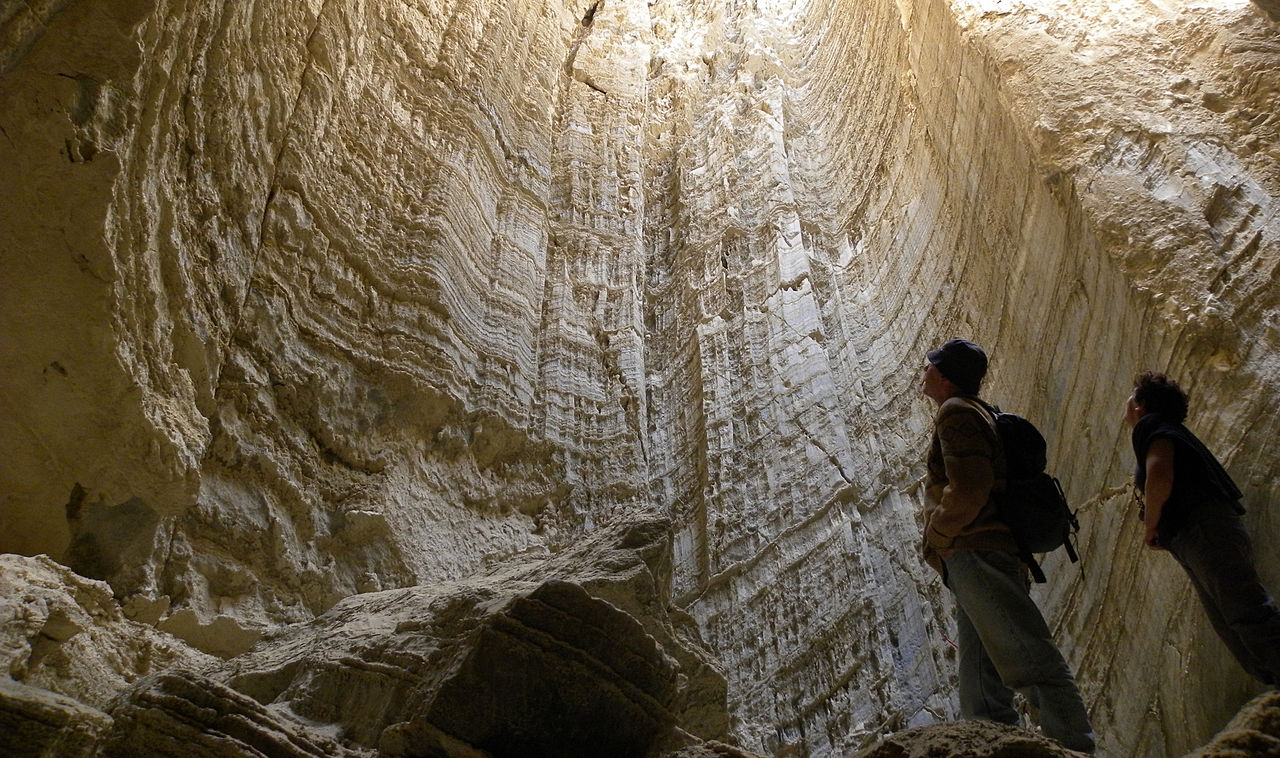
\includegraphics[height=2.5cm]{surface_types/salt.jpg}\\
            \caption*{Salt}
            \label{fig:salt}
        \end{subfigure}
        \hfill
        \begin{subfigure}[b]{0.3\textwidth}
            \centering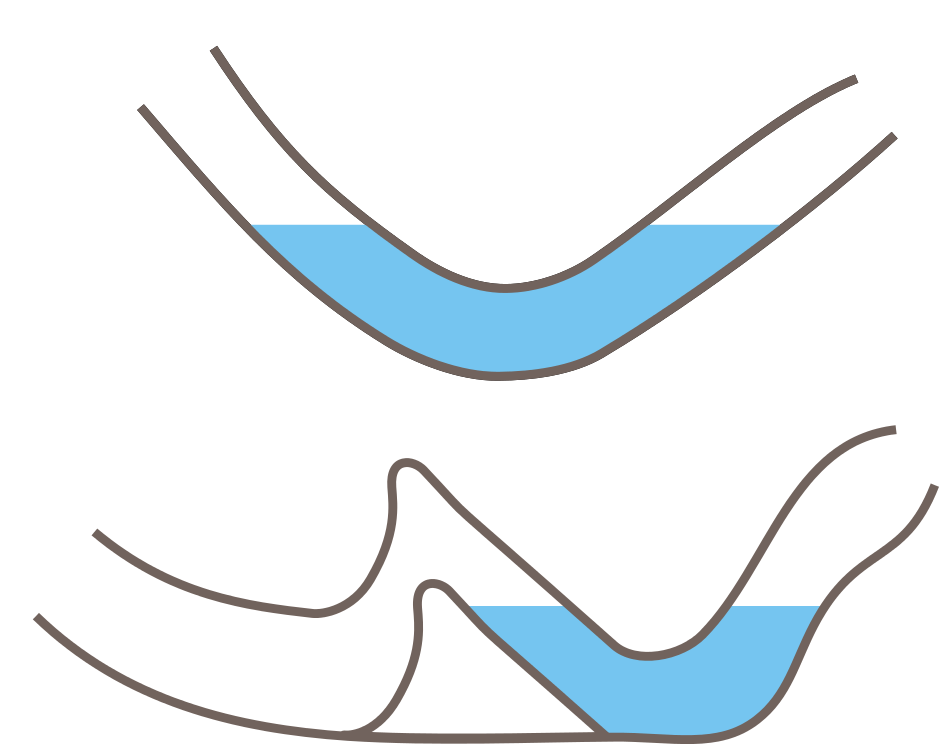
\includegraphics[height=2.5cm]{surface_types/siphon.png}\\
            \caption*{Siphon}
            \label{fig:siphon}
        \end{subfigure}
        \hfill
        \begin{subfigure}[b]{0.3\textwidth}
            \centering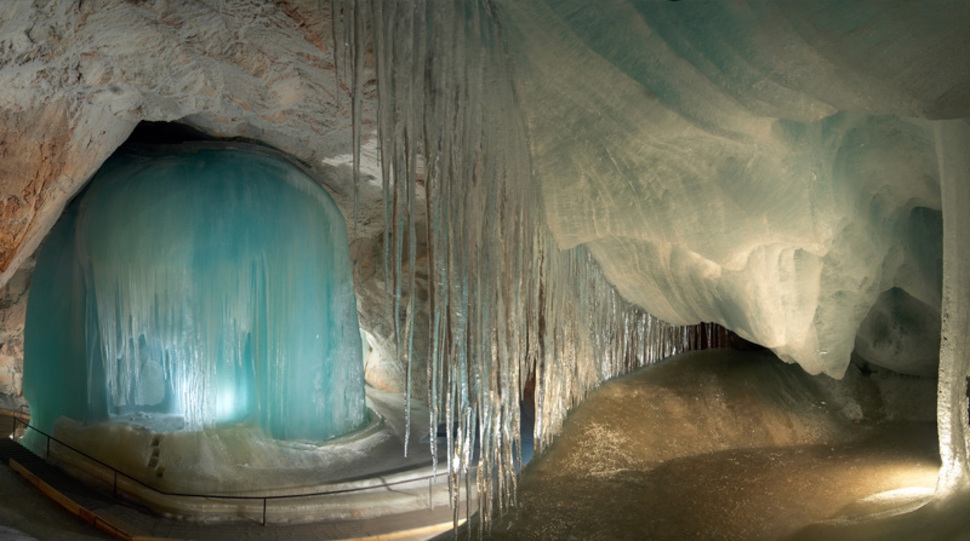
\includegraphics[height=2.5cm]{surface_types/ice.png}\\
            \caption*{Glacier cave}
            \label{fig:ice}
        \end{subfigure}

        \begin{subfigure}[b]{0.3\textwidth}
            \centering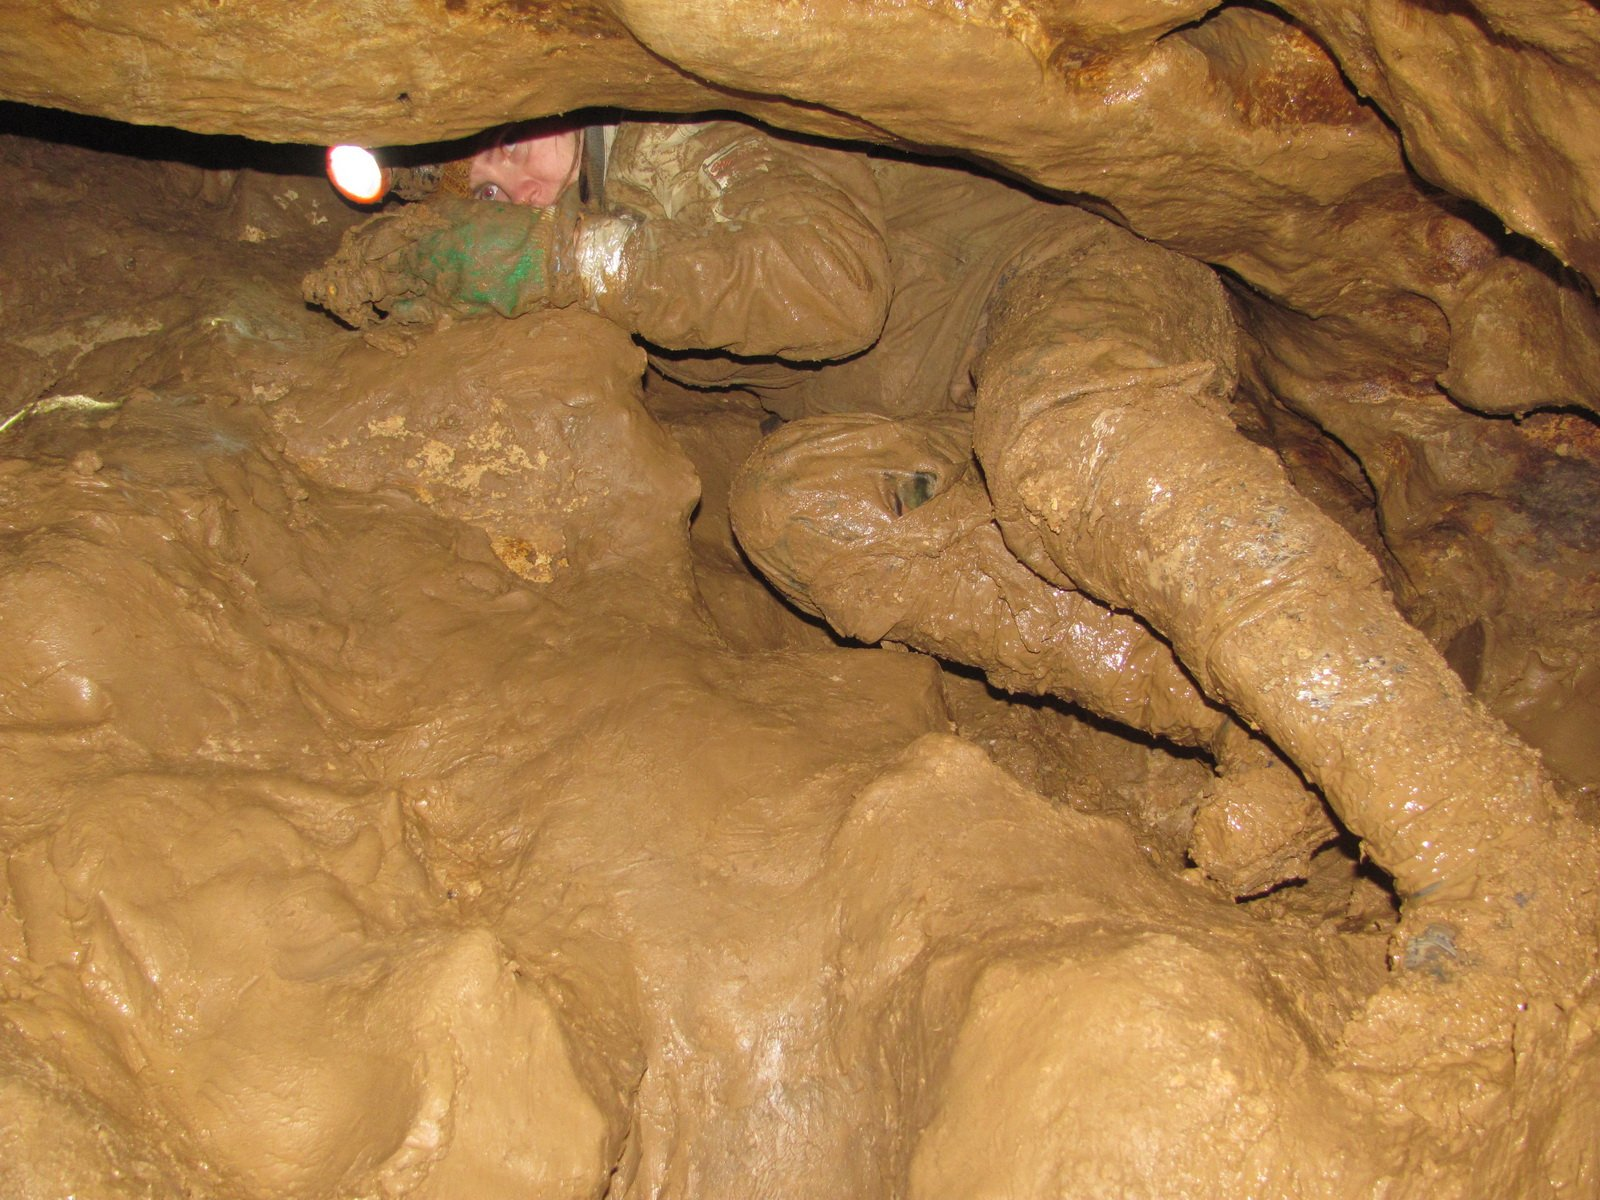
\includegraphics[height=2.5cm]{surface_types/clay.jpg}\\
            \caption*{Clay}
            \label{fig:clay}
        \end{subfigure}
        \hfill
        \begin{subfigure}[b]{0.3\textwidth}
            \centering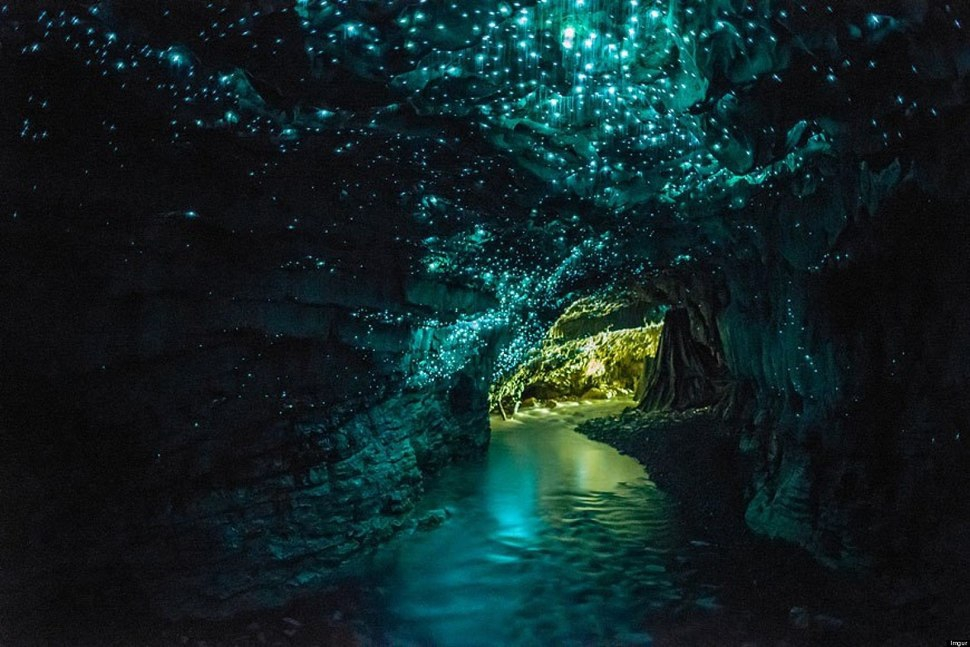
\includegraphics[height=2.5cm]{surface_types/splash.png}\\
            \caption*{Splash}
            \label{fig:splash}
        \end{subfigure}
        \hfill
        \begin{subfigure}[b]{0.3\textwidth}
            \centering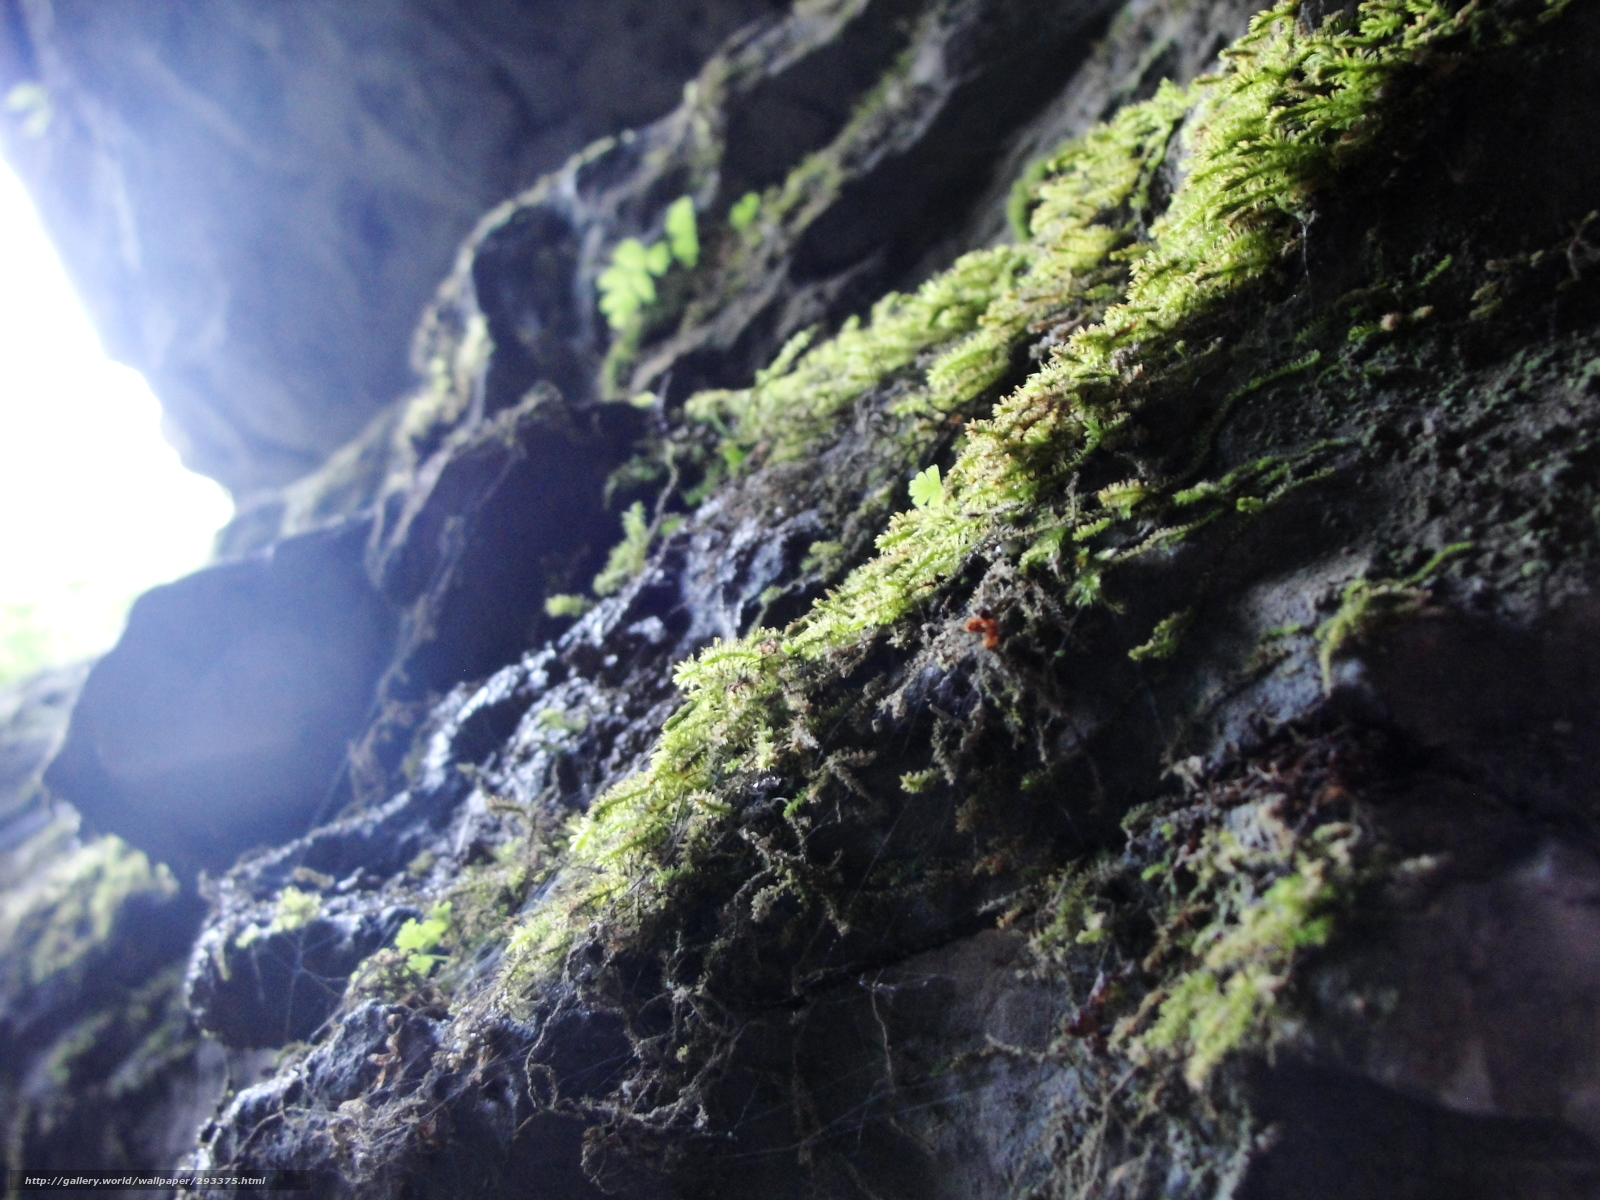
\includegraphics[height=2.5cm]{surface_types/moss.jpg}\\
            \caption*{Moss}
            \label{fig:moss}
        \end{subfigure}
    \end{figure}
\end{frame}

\begin{frame}[t]{Motivation: unsolvable problem for cameras and lidars}
    \framesubtitle{Question: how to make a terrain map when you have a spash above?}
    \vspace{-1cm}
    \begin{columns}[T,onlytextwidth]
        \begin{column}{0.55\textwidth}
            \begin{figure}[H]
                \centering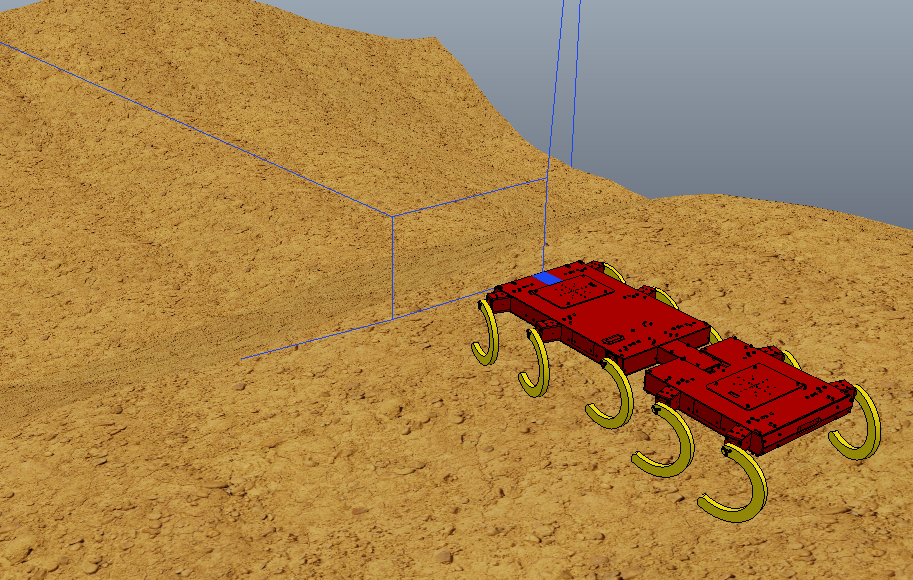
\includegraphics[height=6cm,width=1\textwidth,keepaspectratio]{terrain_wo_water.png}
                \caption*{Terrain without water}
            \end{figure}
        \end{column}
        \begin{column}{0.44\textwidth}
            \begin{figure}[H]
                \begin{subfigure}[b]{0.8\textwidth}
                    \centering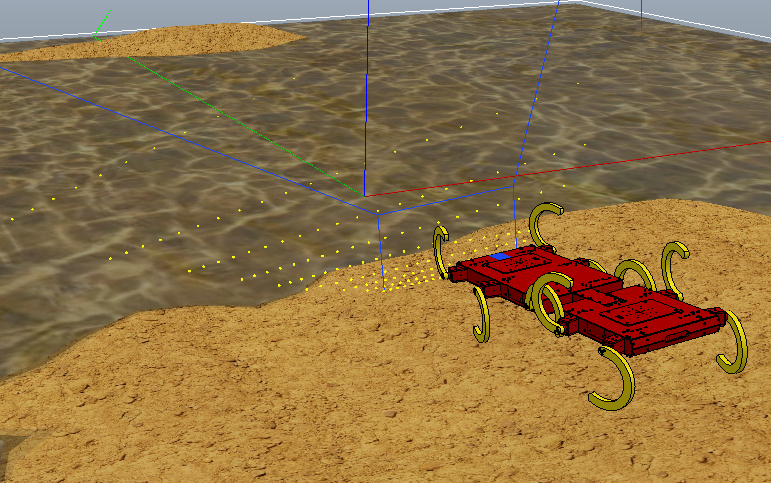
\includegraphics[height=3.5cm,width=1\textwidth,keepaspectratio]{terrain_w_water1.png}
                    % \caption*{Terrain with water, \\ lidar data}
                \end{subfigure}

                \begin{subfigure}{0.8\textwidth}
                    \centering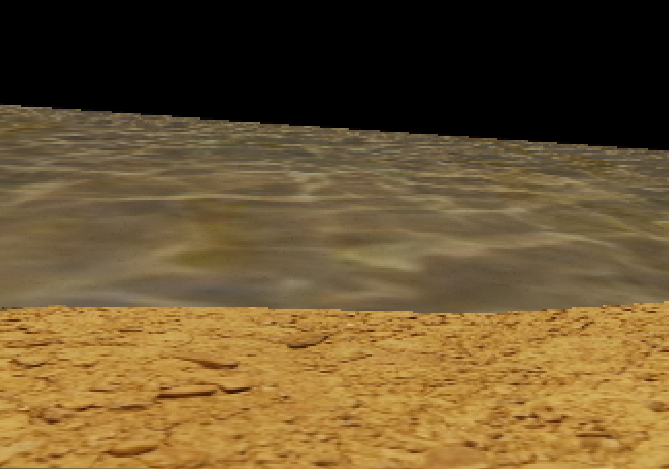
\includegraphics[height=2cm,width=1\textwidth,keepaspectratio]{terrain_w_water_camera.png}
                    \caption*{Camera view}
                \end{subfigure}
            \end{figure}
        \end{column}
    \end{columns}

\end{frame}

% \begin{frame}[t]{Problem statement}
%     \framesubtitle{}
%     \begin{columns}[T,onlytextwidth]
%         \begin{column}{0.45\textwidth}
%             \begin{block}{Problem 1}
%                 How to obtain a useful information about terrain, \textbf{when we have a SLAM based on lidars, cameras}?
%                 \vspace{5pt}

%                 \uncover<2->{\alert{\Large Obtain map and type of terrain}}
%             \end{block}
%         \end{column}
%         \begin{column}{0.45\textwidth}
%             \begin{block}{Problem 2}
%                 How to obtain a useful information about terrain,\textbf{ when main navigation system died}?
%                 \vspace{5pt}

%                 \uncover<2->{\alert{\Large Problem 1 + localization}}
%             \end{block}
%         \end{column}
%     \end{columns}
% \end{frame}

\begin{frame}[t]{Problem statement}
    \framesubtitle{}
    \begin{block}{Problem 1}
        \Large
        How to obtain a useful information about terrain, \textbf{when we have a SLAM based on lidars, cameras}?
        \vspace{5pt}

        \uncover<2->{\alert{\Large Obtain map and type of terrain}}
    \end{block}
\end{frame}

\begin{frame}[t]{Proposed solutions}
    \framesubtitle{}
    \begin{exampleblock}{Problem 1}
        \Large
        \textit{Map can be built} \textbf{using tactile sensors} on each leg of the robot and create a \textbf{dense point cloud} using sampling from generated mesh using \textbf{modified Delaunay triangulation}.
        \vspace{5pt}

        \textit{Terrain type} can be obtained solving \textbf{terrain classification} problem using \textbf{machine learning}.
    \end{exampleblock}
\end{frame}

% \begin{frame}[t]{Proposed solutions}
%     \framesubtitle{}
%     \begin{columns}[T,onlytextwidth]
%         \begin{column}{0.45\textwidth}
%             \begin{exampleblock}{Problem 1}
%                 \textit{Map can be built} \textbf{using tactile sensors} on each leg of the robot and create a \textbf{dense point cloud} using sampling from generated mesh using \textbf{modified Delaunay triangulation}.
%                 \vspace{5pt}

%                 \textit{Terrain type} can be obtained solving \textbf{terrain classification} problem using \textbf{machine learning}.
%             \end{exampleblock}
%         \end{column}
%         \begin{column}{0.45\textwidth}
%             \begin{exampleblock}{Problem 2}
%                 \textit{Localization problem} can be solved by \textbf{fused data} from net of \textbf{beacons} plus \textbf{several IMU} on board and knowing a \textbf{kinematics} of the system.
%             \end{exampleblock}
%         \end{column}
%     \end{columns}
% \end{frame}



\begin{frame}[t]{Literature review}
    \framesubtitle{}
    \Large
    I searched about:
    \begin{itemize}
        \item Cave environment: obstacles, dimensions.
        \item Robots for cave exploration. From zeppelins, to quadruped robots.
        \item Methods for map creation using classical way and haptic. Based on cameras, lidars, tactile sensors and etc.
    \end{itemize}
    \begin{block}{Summary}
        I haven't found any paper, who tried to create a map using tactile sensors in a cave.
    \end{block}
\end{frame}

\begin{frame}[t]{Robot design}
    \framesubtitle{Requirements}
    \Large
    \textbf{Problem} --  choose robot mover type. This robot should:
    \begin{itemize}
        \item should have \textit{small dimensions} to sneak through holes;
        \item have enough \textit{mobility} to pass a granular terrain;
        \item should \textit{pass a small water obstacles};
        \item can \textit{climb on a big stones};
    \end{itemize}
    \uncover<2->{\LARGE\centering\alert{1-DoF multilegged robot}}
\end{frame}

\begin{frame}[t]{Robot design}
    \framesubtitle{Structural synthesis problem}
    \only<1-2>{\LARGE\begin{block}{Question}
            What the optimal amount of legs should be in such robot?
        \end{block}}
    \only<2>{\LARGE\begin{alertblock}{Answer}
            \centering Robot should have \textbf{10-12 legs} in total!
        \end{alertblock}}
\end{frame}

\begin{frame}[c]{Robot design}
    \framesubtitle{Technological stack}
    \vspace{-1.2cm}
    \begin{figure}[H]
        \begin{subfigure}{0.32\textwidth}
            \centering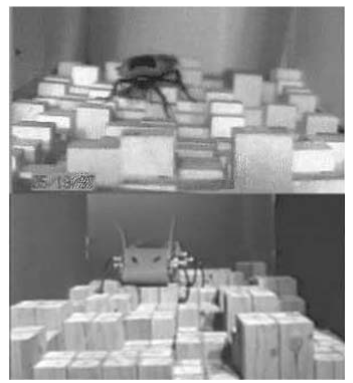
\includegraphics[height=4cm,width=1\textwidth,keepaspectratio]{c1_paper.png}
            \caption*{Generating terrain approach}
        \end{subfigure}
        \hfill
        \begin{subfigure}{0.32\textwidth}
            \centering
\includegraphics[height=4cm,width=1\textwidth,keepaspectratio]{gazebo_logo.png}
            \caption*{Robot simulator}
        \end{subfigure}
        \hfill
        \begin{subfigure}{0.32\textwidth}
            \centering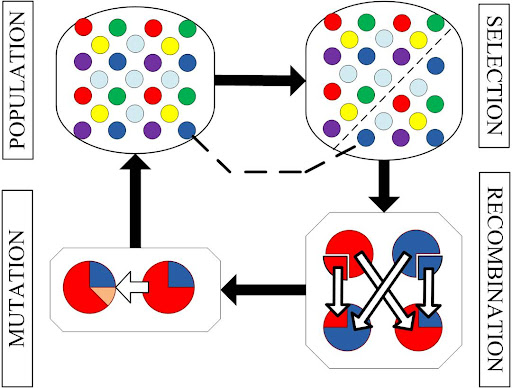
\includegraphics[height=5.5cm,width=1\textwidth,keepaspectratio]{gen_algo.jpg}
            \caption*{Genetic algorithm \\ (DEAP Library)}
        \end{subfigure}
        \hfill
    \end{figure}
\end{frame}

\begin{frame}[t]{Robot design}
    \framesubtitle{Proposed solution}
    \begin{columns}[T,onlytextwidth]
        \begin{column}{0.49\textwidth}
            \begin{figure}[H]
                \centering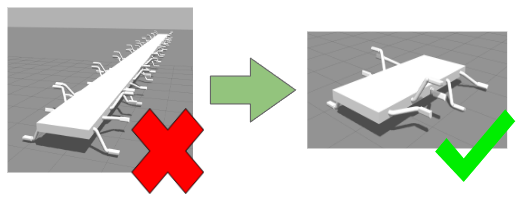
\includegraphics[height=3cm,width=1\textwidth,keepaspectratio]{optimization_idea.png}
                \caption*{\textbf{Idea}: Minimize number of legs without losing cross-road passability}
                \label{fig{optimization_idea.png}}
            \end{figure}
        \end{column}
        \begin{column}{0.49\textwidth}
            \begin{eqnarray*}
                F = \beta \left( {\omega}_{1} \cdot \overbrace{\delta}^{\text{Distance}} + {\omega}_{2} \cdot \overbrace{\frac{1}{(\gamma - 1) sin(x)}}^{\text{Body length}}\right) +\\ \nonumber + (1 - \beta) {\delta}^{{\omega}_{1}} {\left( \frac{1}{(\gamma - 1) sin(x)}\right)}^{{\omega}_{2}}
            \end{eqnarray*}
            \vspace{1pt}

            $\beta$ is adaptive parameter, ${\omega}_{1,2}$ are the weight coefficients.
        \end{column}
    \end{columns}
\end{frame}

\begin{frame}[t]{Robot design}
    \framesubtitle{Video: the story of one generated robot}
    \vspace{-0.6cm}
    \begin{figure}[H]
        \href{run:./videos/pass_rand_terr.mp4}{
            \centering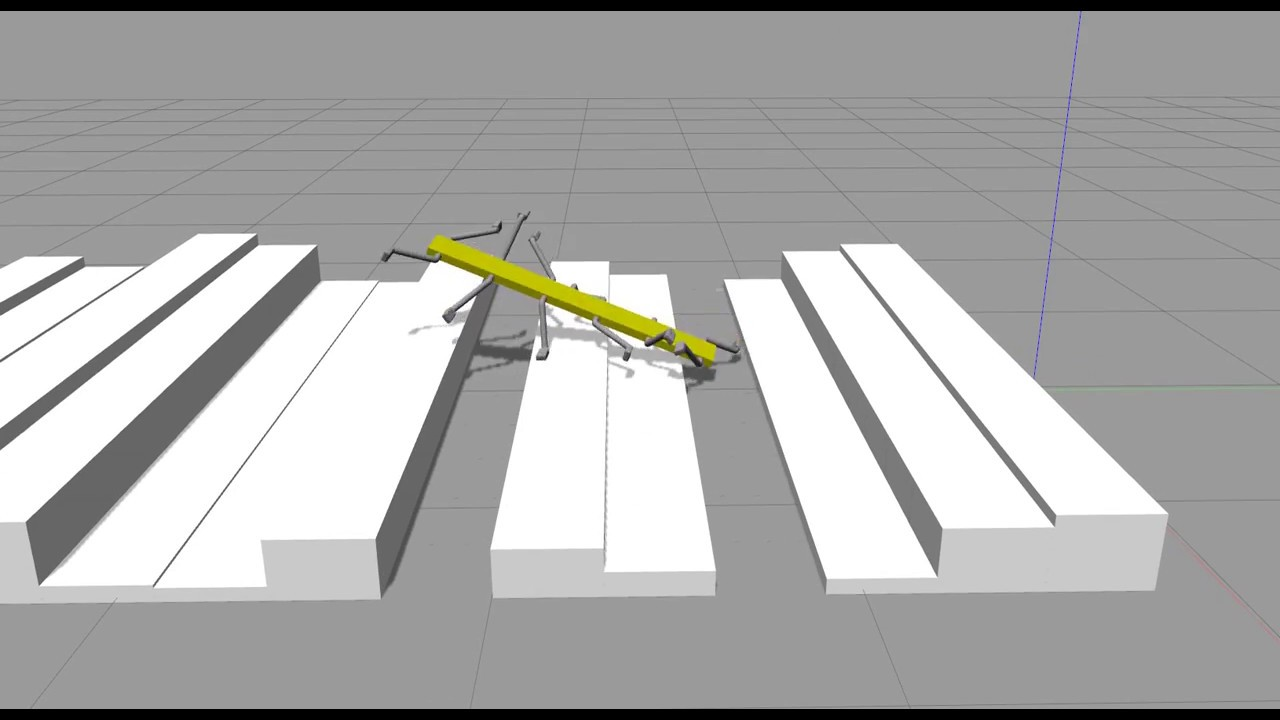
\includegraphics[height=6cm,width=1\textwidth,keepaspectratio]{genetic_video_preview.jpg}}
        % \caption{Click on a picture for a video}
    \end{figure}
\end{frame}

\begin{frame}[t]{Robot design}
    \framesubtitle{Results}
    \vspace{-0.5cm}
    \begin{figure}[H]
        \centering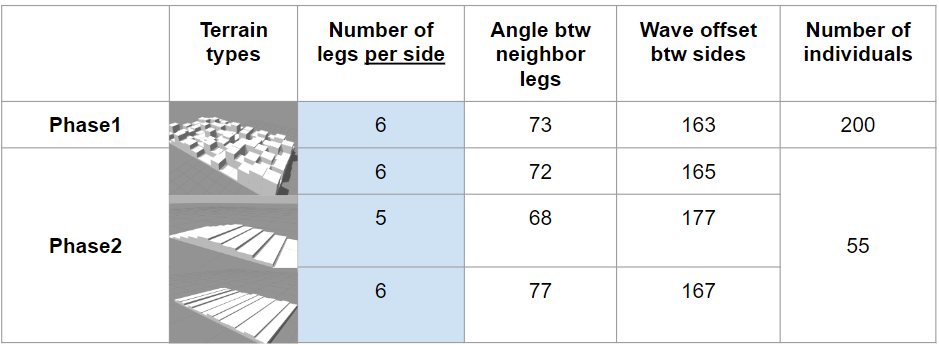
\includegraphics[height=5.5cm,width=1\textwidth,keepaspectratio]{table_terrain.png}
        \caption*{\LARGE\centering\textbf{Summary}: robot should have 10-12 legs in total}
        \label{fig:table_terrain.png}
    \end{figure}
\end{frame}

\begin{frame}[t]{Robot design}
    \framesubtitle{Increasing maneuverablity}
    \only<1-2>{\Large\begin{block}{Question}
            1. Long robot can stuck in a cave hole, while rotating. How to avoid it?

            2. How to climb on big stones?
        \end{block}}
    \only<2>{\Large\begin{alertblock}{Answer}
            \centering 1. Add an ability to sidestep without changing orientation.

            2. Make a segmented body.
        \end{alertblock}}
\end{frame}

\begin{frame}[t]{Robot design}
    \framesubtitle{Video}
    \vspace{-0.6cm}
    \begin{figure}[H]
        \href{run:./videos/sidestep_segments.mp4}{
            \centering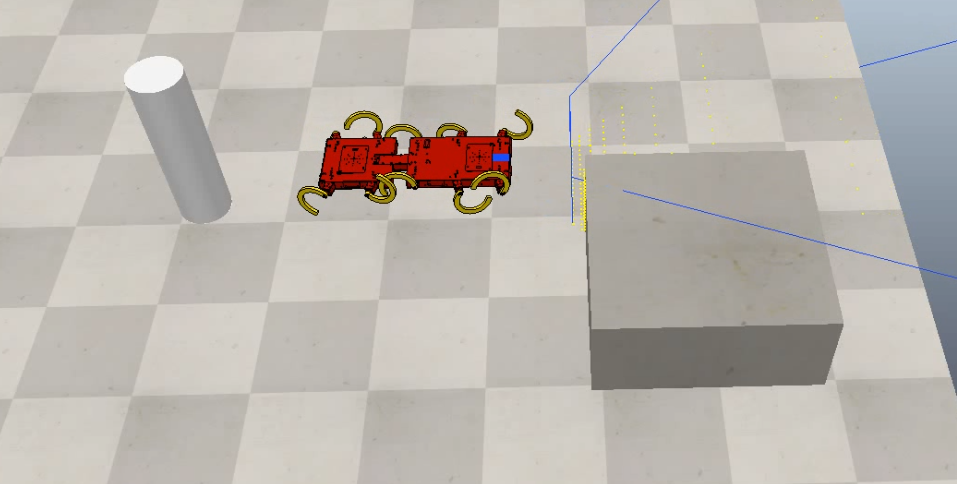
\includegraphics[height=6cm,width=1\textwidth,keepaspectratio]{sidestep_segment_video_preview.png}}
        % \caption{Click on a picture for a video}
    \end{figure}
\end{frame}

\begin{frame}[t]{Robot design}
    \framesubtitle{Proposed solution}
    \vspace{-0.8cm}
    \begin{figure}[H]
        \centering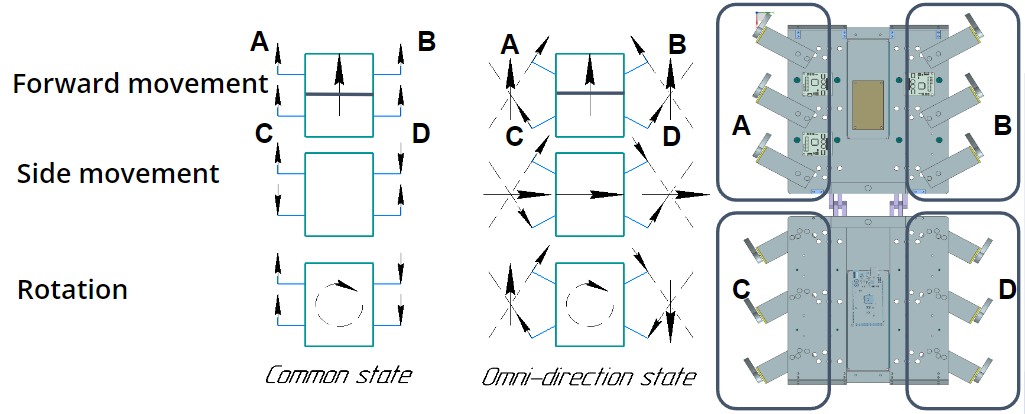
\includegraphics[height=5.5cm,width=1\textwidth,keepaspectratio]{omni_rot.png}
        \caption*{Vector representation of forces in  the conventional and omni-direction states}
    \end{figure}
\end{frame}

\begin{frame}[t]{Robot design}
    \framesubtitle{StriRus prototypes (1)}
    \vspace{-0.7cm}
    \begin{figure}[H]
        \begin{subfigure}[t]{0.32\textwidth}
            \centering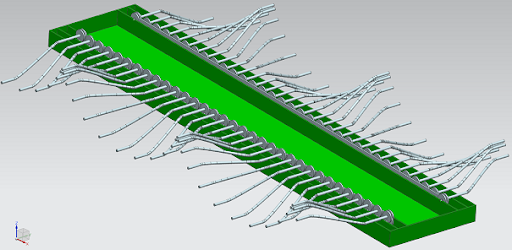
\includegraphics[height=4cm,width=1\textwidth,keepaspectratio]{strirus_0.png}
            \caption*{\textbf{1st gen}: 54 legs \\ 1 segment}
        \end{subfigure}
        \hfill
        \begin{subfigure}[t]{0.32\textwidth}
            \centering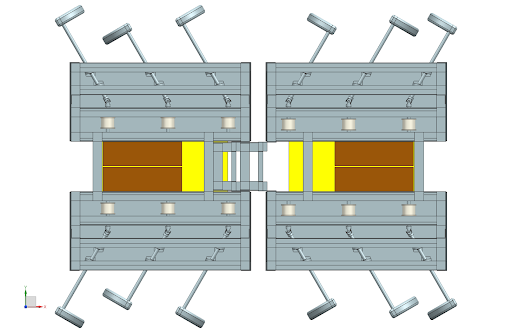
\includegraphics[height=4cm,width=1\textwidth,keepaspectratio]{strirus_1.png}
            \caption*{\textbf{2nd gen}: 12 legs \\ 2 segments, 1 DoF connection \\ Continuous angle b/w body, leg up to 45 deg}
        \end{subfigure}
        \hfill
        \begin{subfigure}[t]{0.32\textwidth}
            \centering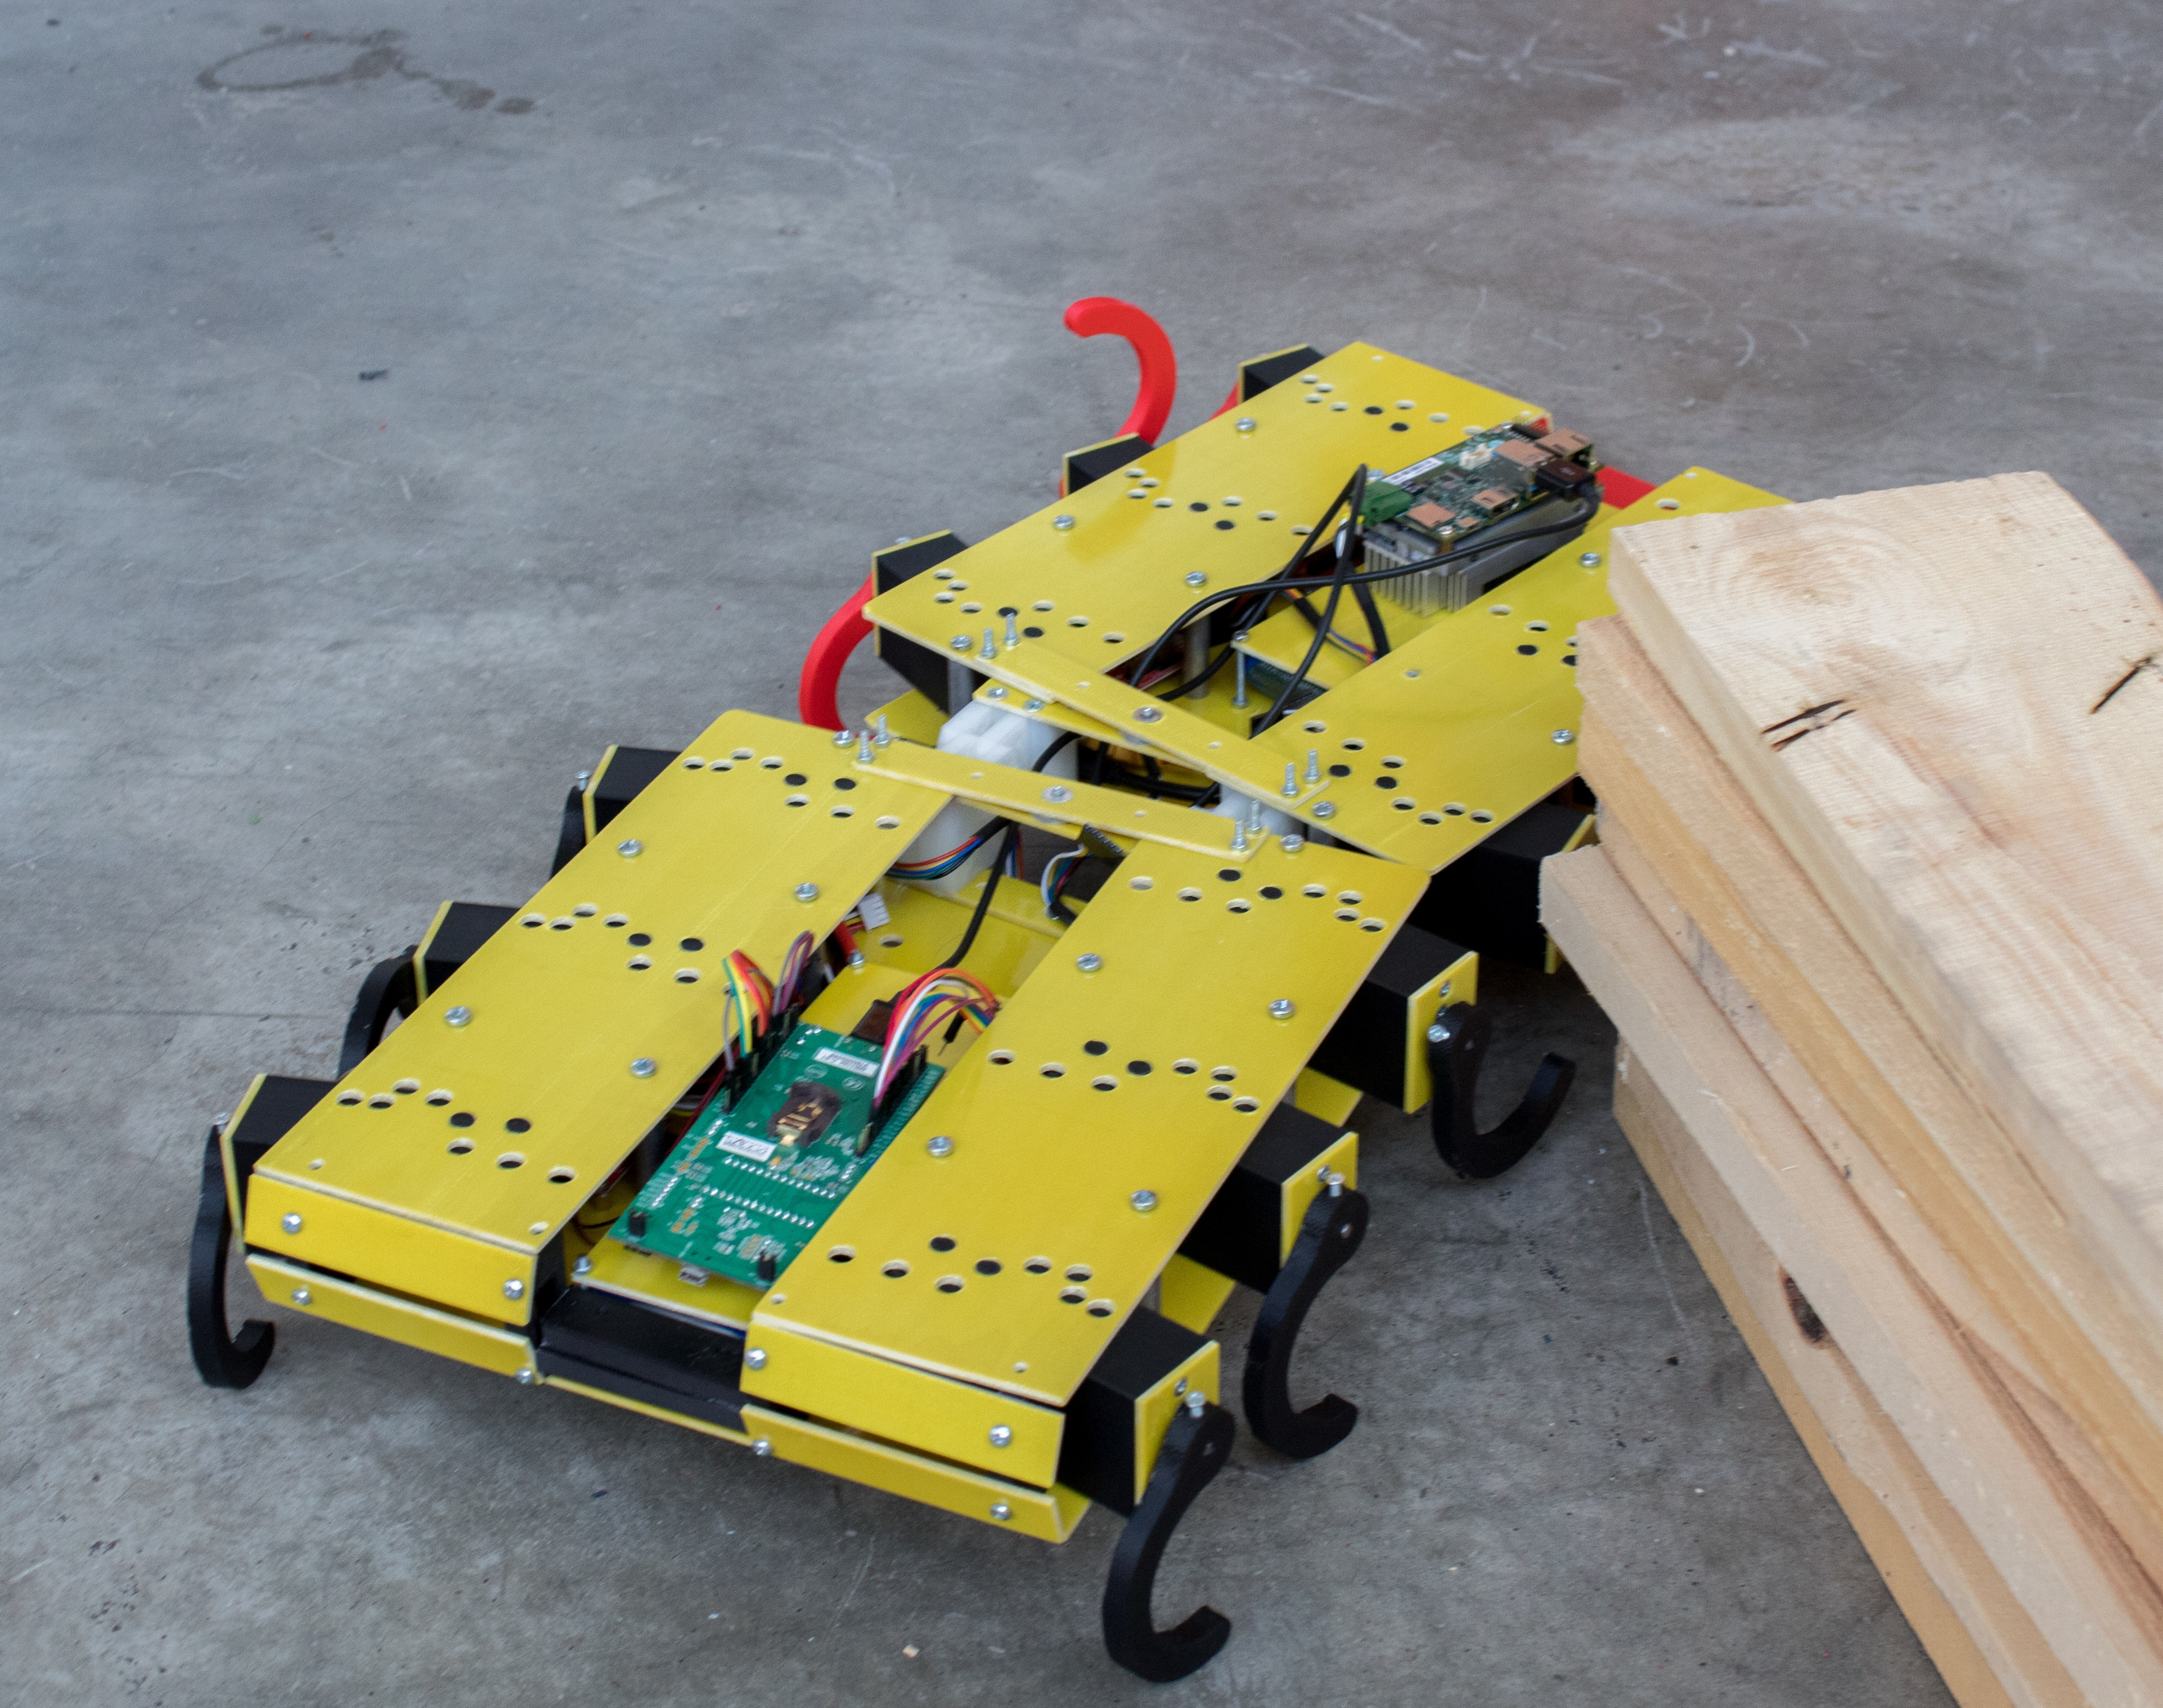
\includegraphics[height=4cm,width=1\textwidth,keepaspectratio]{strirus_2.jpg}
            \caption*{\textbf{3rd gen}: 12 legs \\ 2 segments, 2 DoF connection \\ Discrete angle b/w body, leg up to 45 deg}
        \end{subfigure}
        \hfill
    \end{figure}
\end{frame}

\begin{frame}[t]{Robot design}
    \framesubtitle{StriRus prototypes (2)}
    \vspace{-0.5cm}
    \begin{figure}[H]
        \begin{subfigure}[t]{0.45\textwidth}
            \centering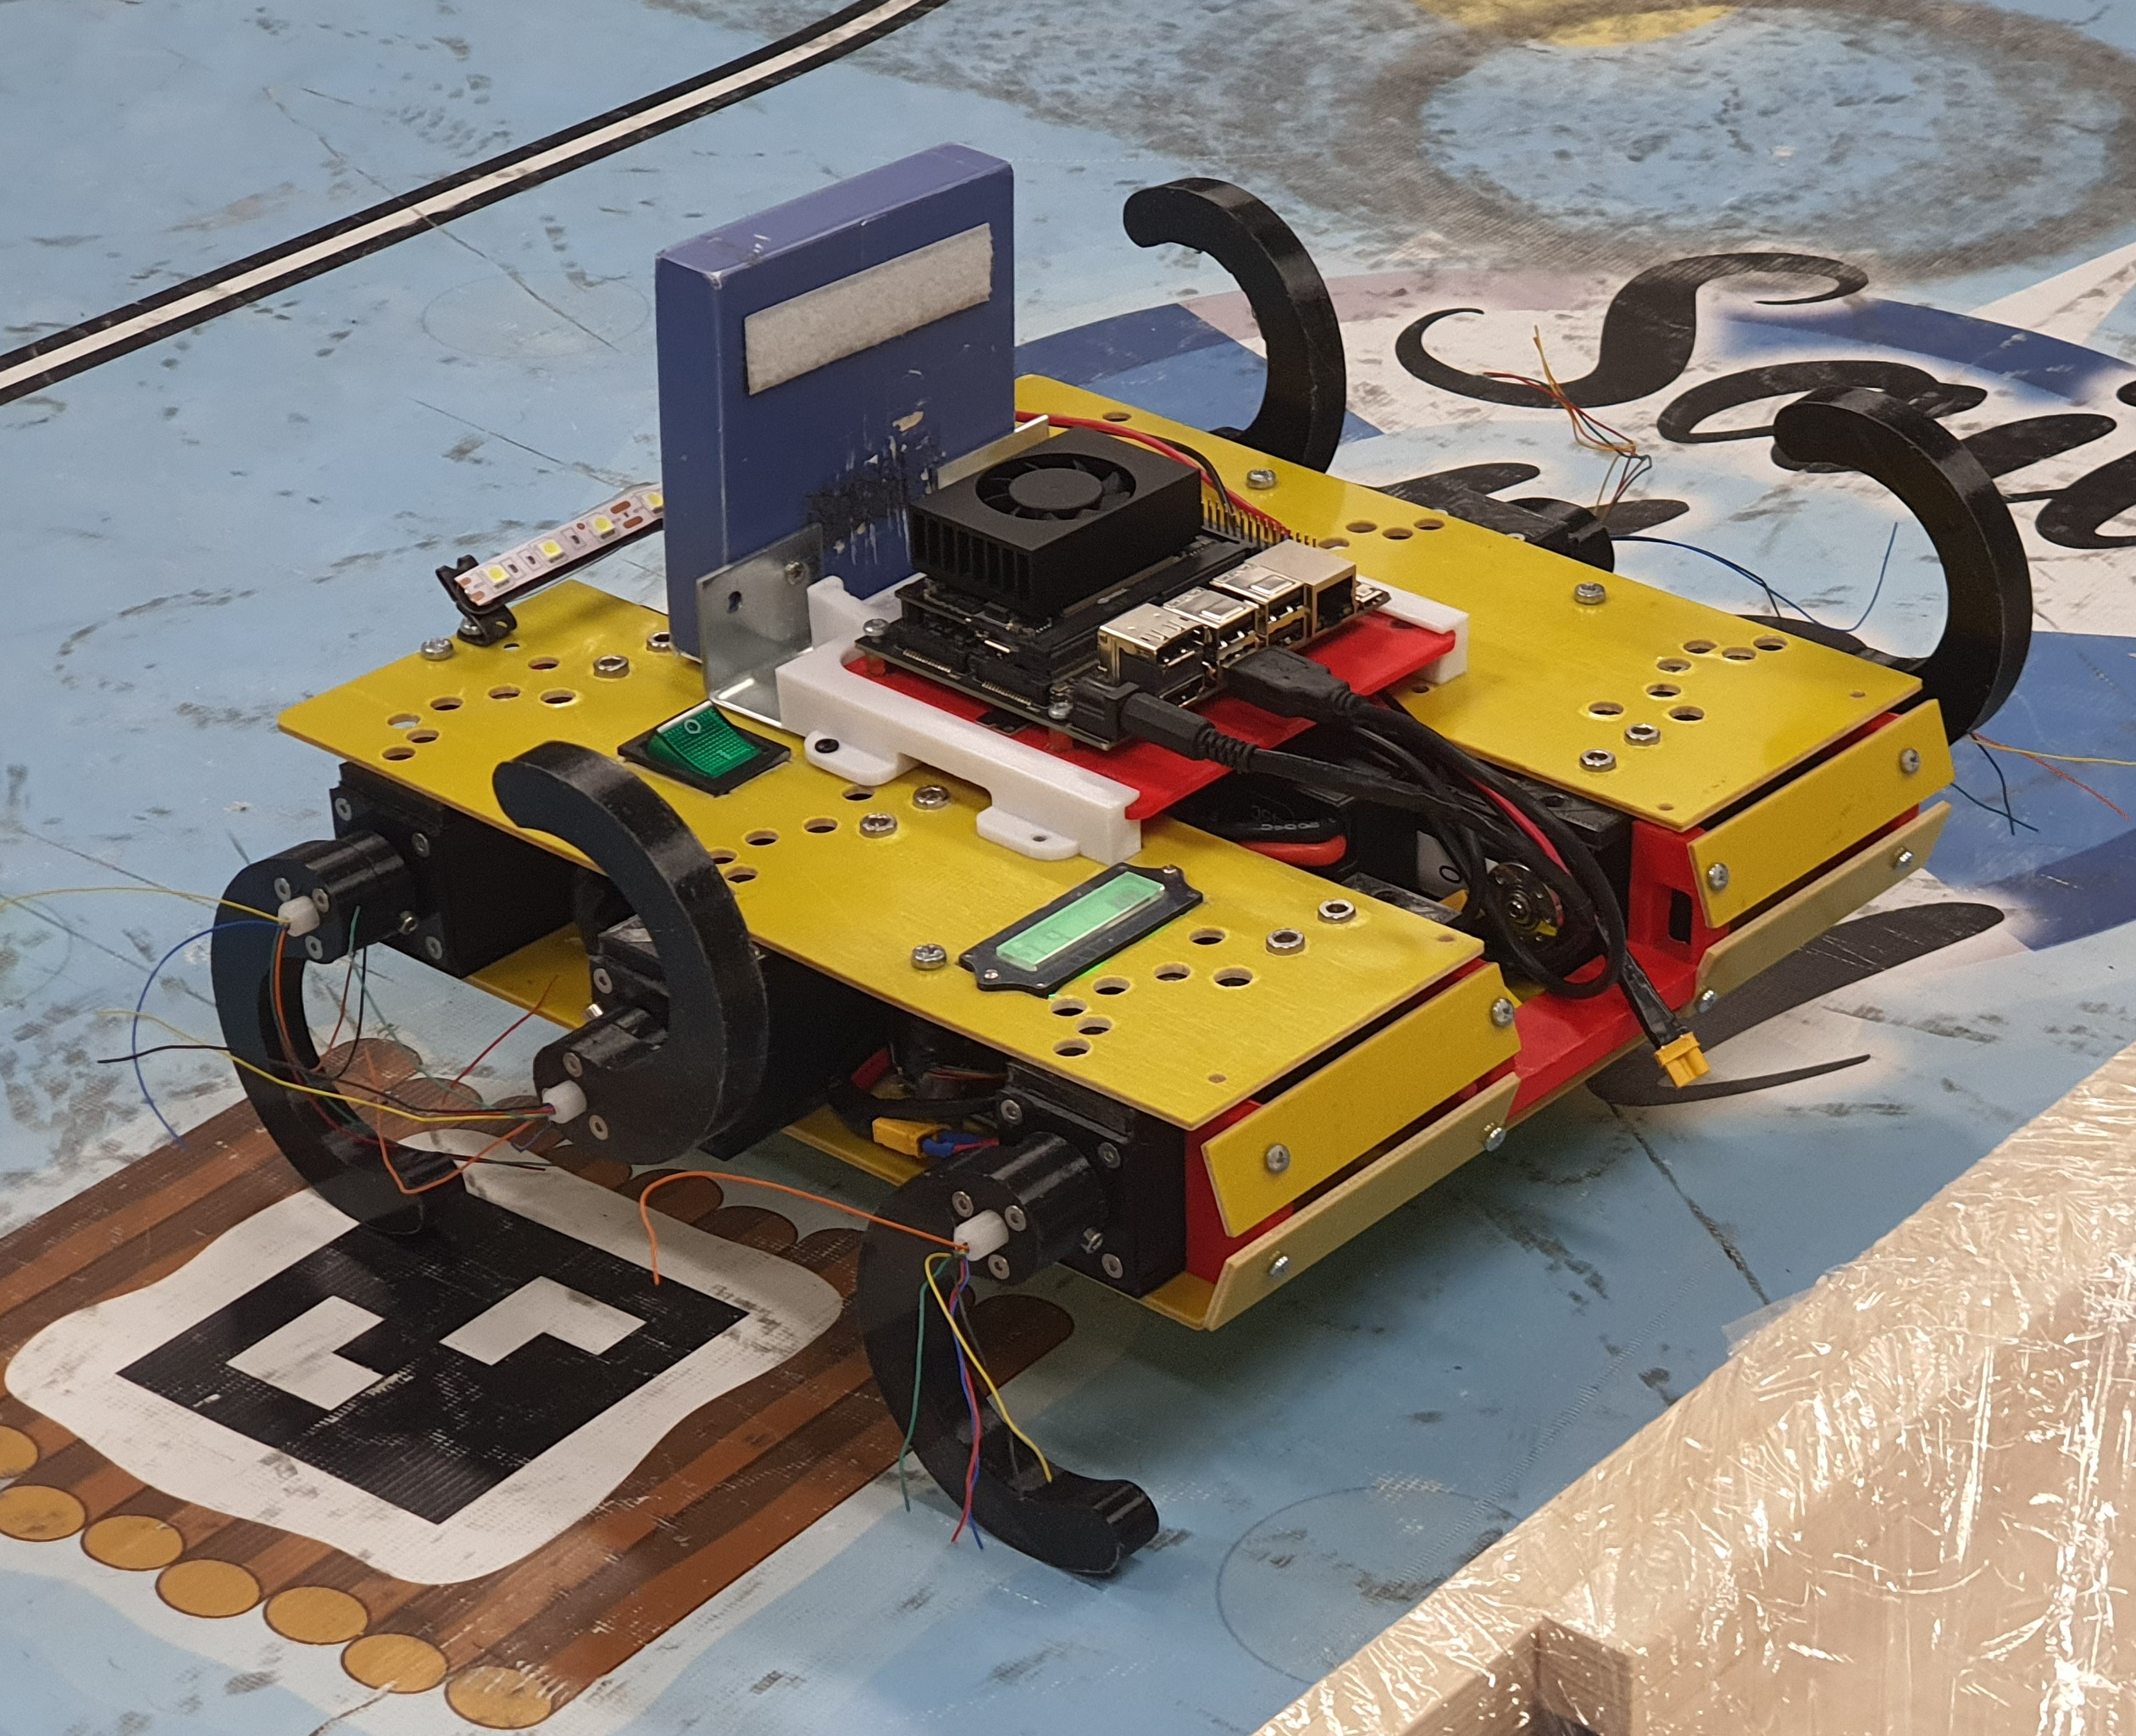
\includegraphics[height=4cm,width=1\textwidth,keepaspectratio]{strirus_3.JPG}
            \caption*{\textbf{3th+ gen}: 6 big legs \\ 1 segment}
        \end{subfigure}
        \hfill
        \begin{subfigure}[t]{0.45\textwidth}
            \centering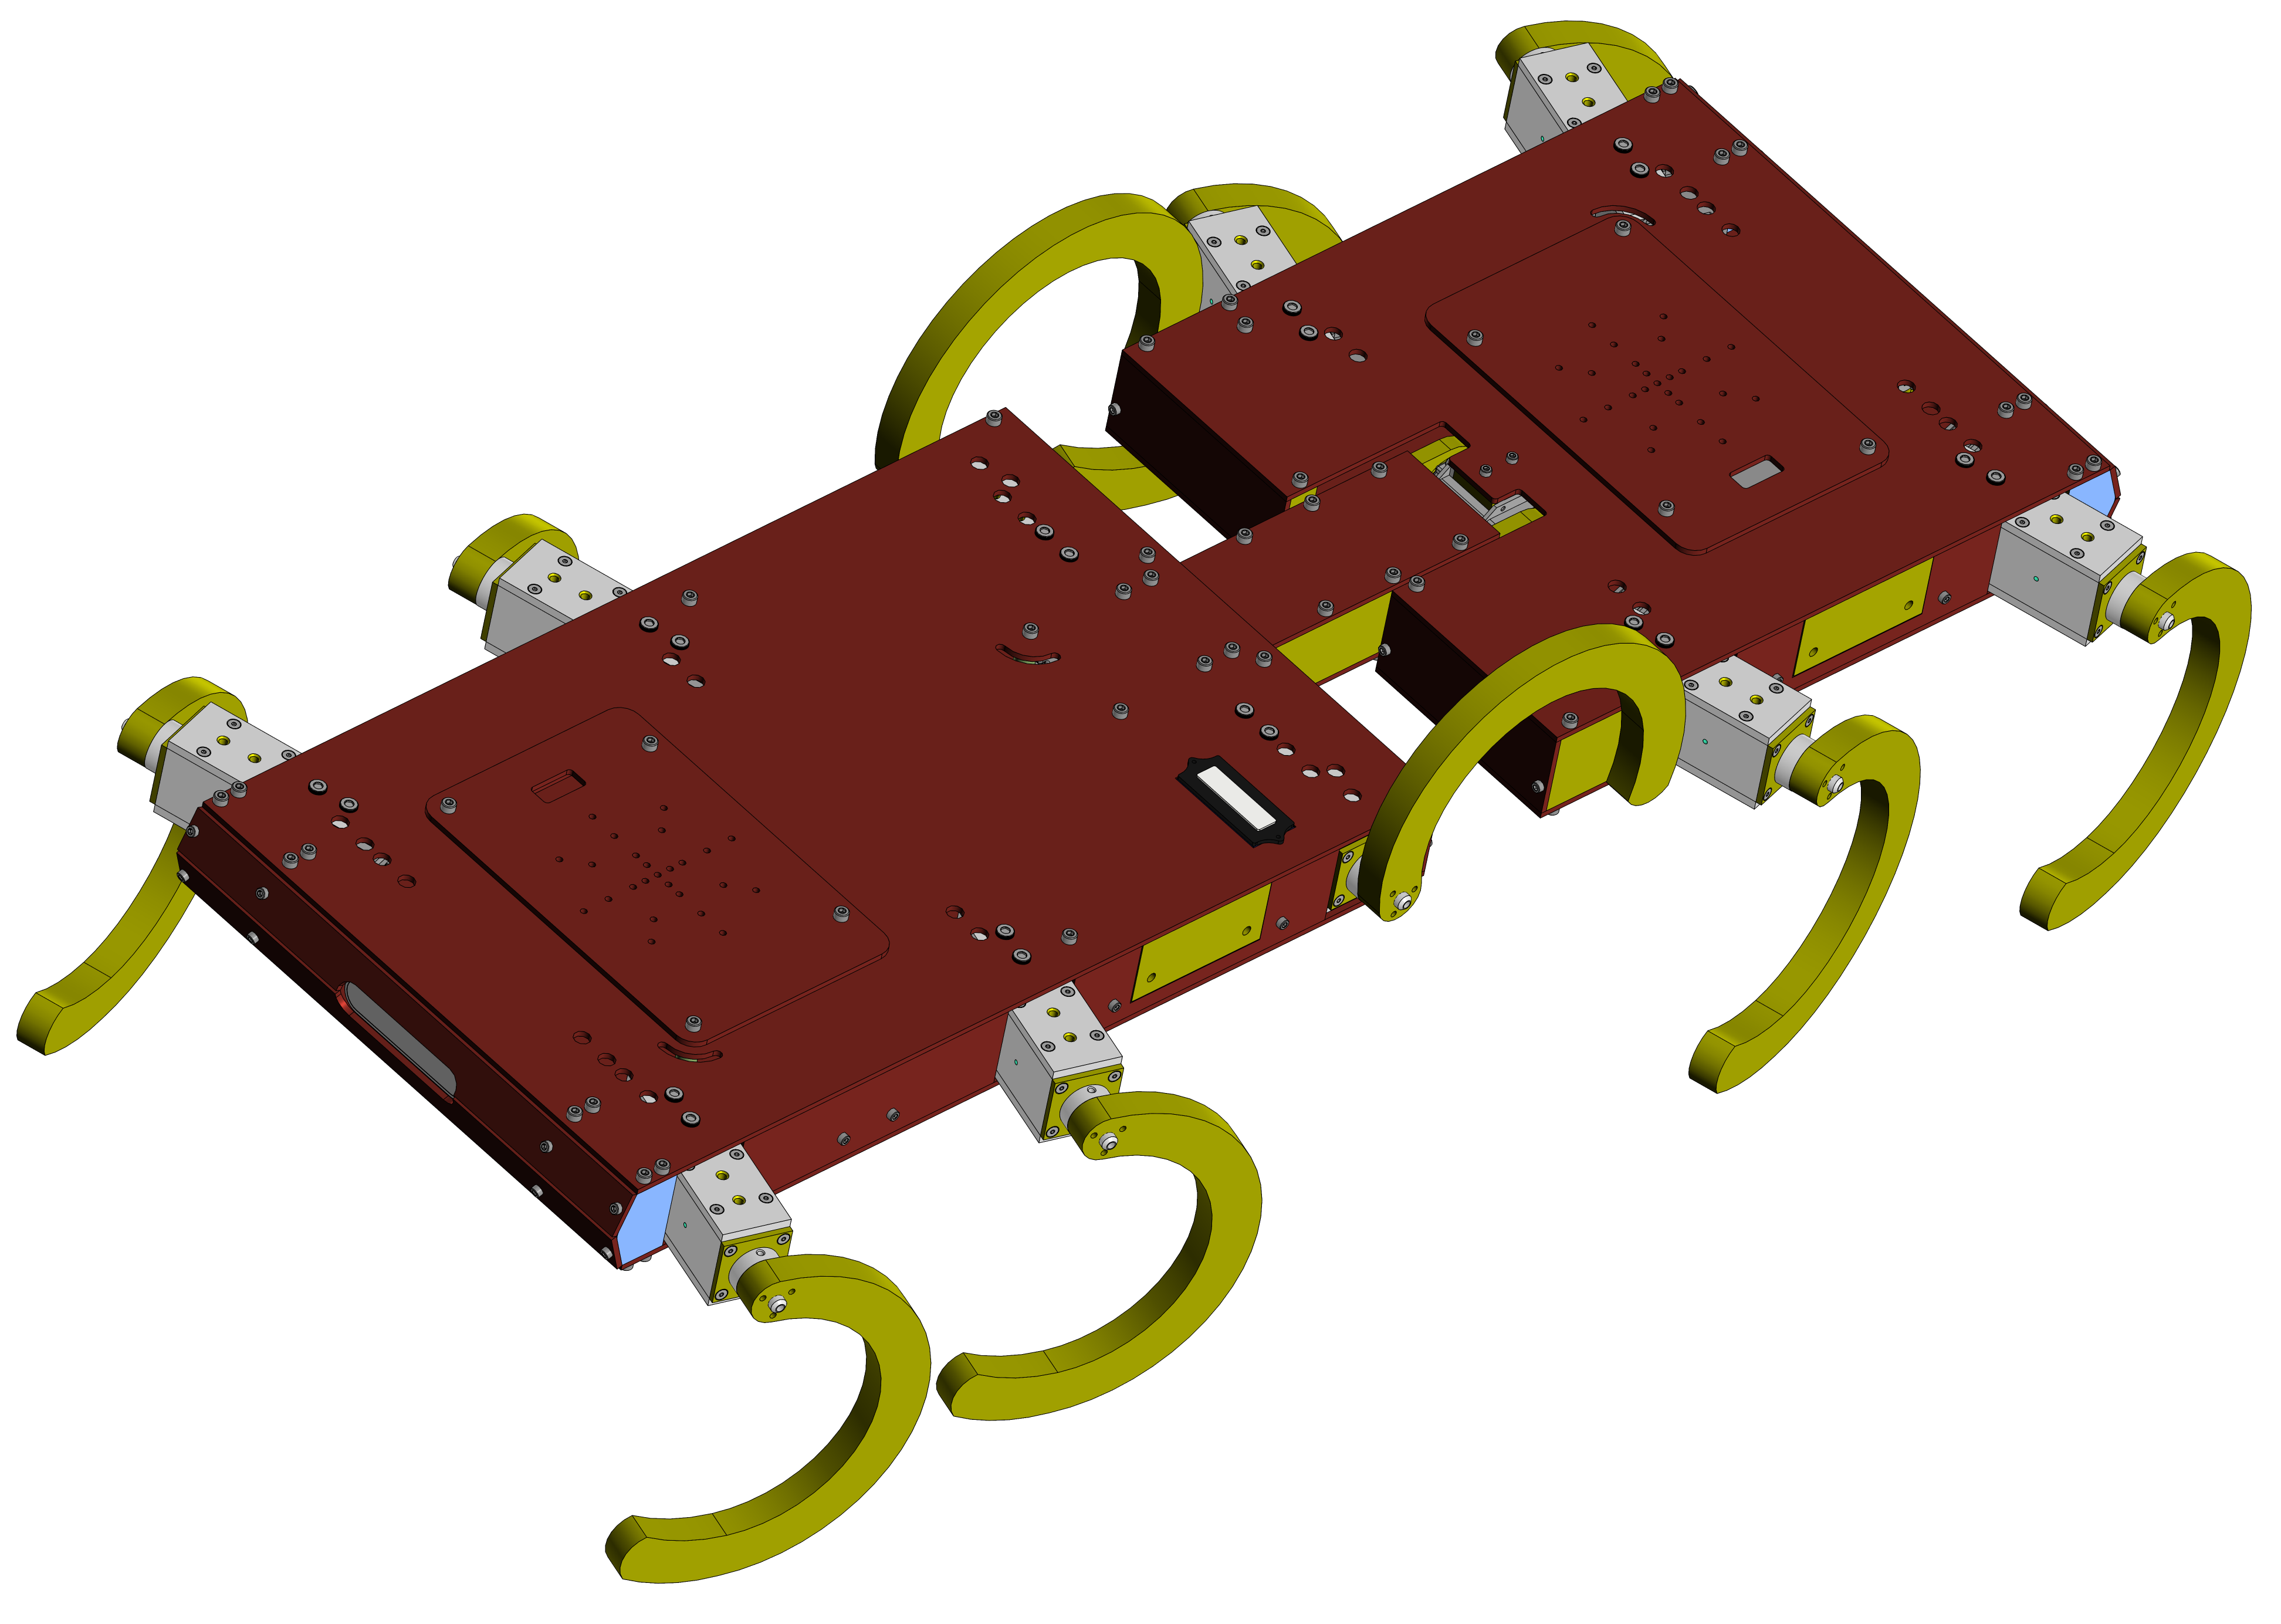
\includegraphics[height=4cm,width=1\textwidth,keepaspectratio]{strirus_4.png}
            \caption*{\textbf{4th gen}: 10 biggest legs \\ 2 segments, 1 DoF connection \\  Discrete angle b/w body, leg up to 15 deg}
        \end{subfigure}
        \hfill
    \end{figure}
\end{frame}

\begin{frame}[t]{Force transducer design}
    \framesubtitle{}
    \only<1-2>{\LARGE\begin{block}{Question}
            How to receive a reaction force from the ground?
        \end{block}}
    \only<2>{\LARGE\begin{alertblock}{Answer}
            \centering Installing a force sensor on each leg
        \end{alertblock}}
\end{frame}

\begin{frame}[t]{Force transducer design}
    \framesubtitle{Force sensor types}
    \vspace{-20pt}
    \begin{multicols}{2}
        \begin{itemize}
            \item \textbf{F/T sensors}: too big and expencive for small robots.
            \item \textbf{Optical}: too thick.
            \item \textbf{Magnetic}: too thick.
            \item \textbf{Capacitive}: expencive, but the best in terms of requirements.
            \item \textbf{Piezoresistive sensors
                      based on conductive inks or polymers}: inexpencive and robust, but has problems with hysteresis
            \item \textbf{Stain gages}: challenge for wiring between continuously rotating legs and the robot body.
        \end{itemize}
    \end{multicols}
    \vspace{-10pt}
    \begin{exampleblock}{My choice is \textbf{Resistive sensor based on Velostat}}
        It's cheap and it can be made by hand.
    \end{exampleblock}
\end{frame}

\begin{frame}[t]{Force transducer design}
    \framesubtitle{Velostat}
    \vspace{-20pt}
    \begin{columns}[T,onlytextwidth]
        \begin{column}{0.6\textwidth}
            \begin{exampleblock}{Definition}
                The Velostat is a polymer material filled with carbon black.\\
                \textbf{Expected effects}:
                \begin{itemize}
                    \item \underline{Quantum tunnelling} (Precolation) -- Diod is using such effect;
                    \item \underline{Piezoresistive} -- electrical resistivity of semiconductor is changed by mechanical strain;
                    \item \underline{Viscoelasticity} -- material can damp vibrations.
                \end{itemize}
            \end{exampleblock}
        \end{column}
        \begin{column}{0.38\textwidth}
            \vspace{-0.7cm}
            \begin{figure}[H]
                \begin{subfigure}{0.9\textwidth}
                    \centering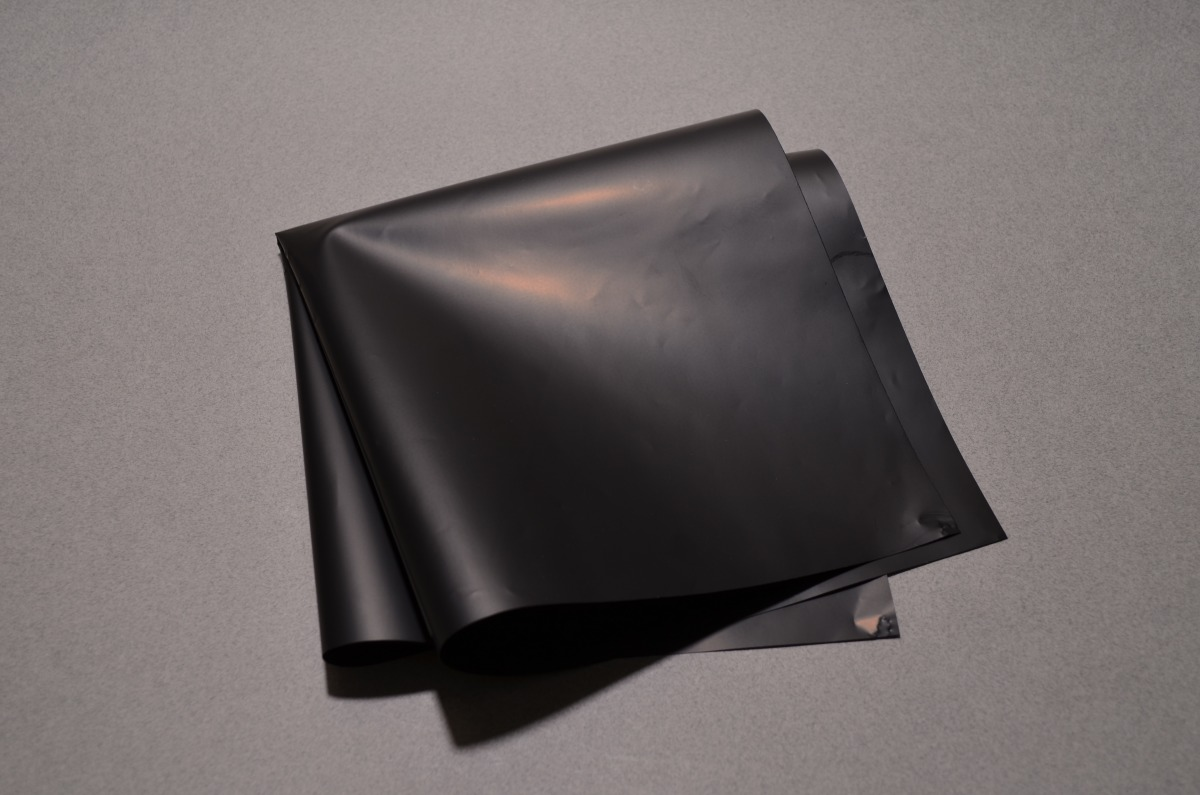
\includegraphics[height=3cm,width=1\textwidth,keepaspectratio]{velostat_sensor.jpg}
                    % \caption*{Velostat material}
                    \label{fig:velostat_sensor.jpg}
                \end{subfigure}

                \begin{subfigure}{0.9\textwidth}
                    \centering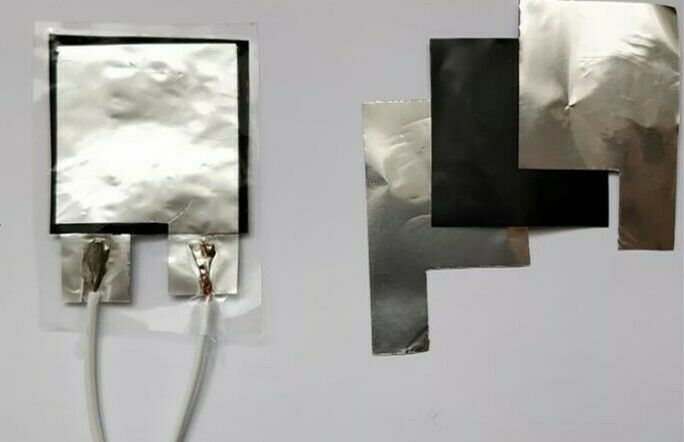
\includegraphics[height=3cm,width=1\textwidth,keepaspectratio]{simplest_sensor.jpg}
                    \caption*{Simplest force transducer}
                    \label{fig:simplest_sensor.jpg}
                \end{subfigure}
            \end{figure}
        \end{column}
    \end{columns}

\end{frame}

\begin{frame}[t]{Force transducer design}
    \framesubtitle{Velostat: Faced problems}
    \vspace{-20pt}
    \begin{multicols}{2}
        {\Large
            \begin{itemize}
                \item Hysteresis
                \item Nonlinearity
                \item Different values with the same pressure if the square of load is less then the sensor
            \end{itemize}}
        \begin{figure}[H]
            \centering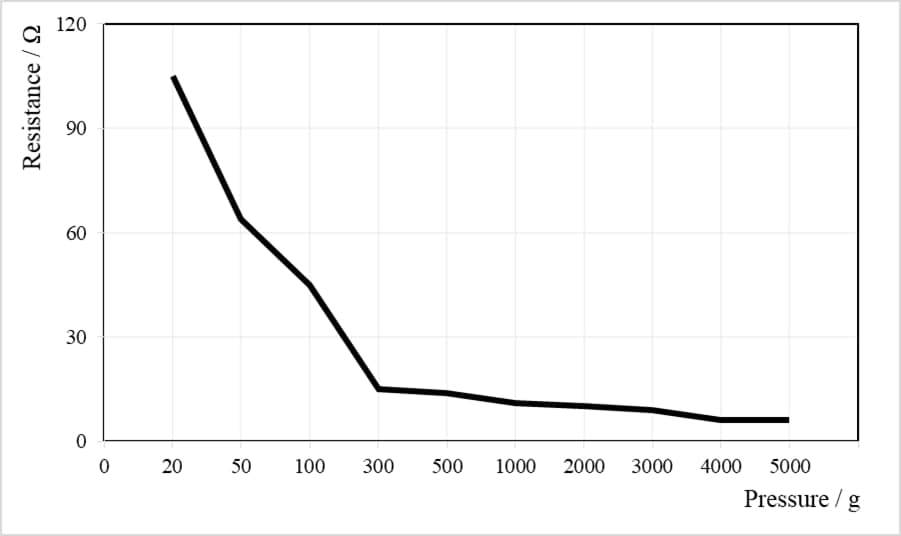
\includegraphics[height=4cm,width=1\textwidth,keepaspectratio]{velostat_pressure_resistance.jpg}
            \label{fig:velostat_pressure_resistance.jpg}
        \end{figure}
    \end{multicols}
    \vspace{-12pt}
    \begin{block}{Scientific Problem Statement}
        To characterize Velostat material for cases when point load is less than sensor size and propose solutions for avoiding such issues.
    \end{block}
\end{frame}

\begin{frame}[t]{Force transducer design}
    \framesubtitle{Experimental setup requirements}
    \vspace{-0.5cm}
    {\Large
        \begin{itemize}
            \item Force control. \only<2>{\alert{Solved by Impedance Control}}
            \item Position and force repeatability. \only<2>{\alert{Solved by adding manipulator and camera}}
            \item To have an ability to apply force only on a part of a sensor. \only<2>{\alert{Solved by adding several end-effectors}}
            \item To change object of the experiment quickly. \only<2>{\alert{Solved by experimental setup}}
        \end{itemize}}
    \only<2>{\centering\Large\alert{All requirements are fulfilled}}
\end{frame}


\begin{frame}[t]{Force transducer design}
    \framesubtitle{Experimental Setup: Hardware overall}
    \vspace{-12pt}
    \begin{center}
    \begin{tikzpicture}

        % Include the image in a node
        \node [
            above right,
            inner sep=0] (image) at (0,0) {\centering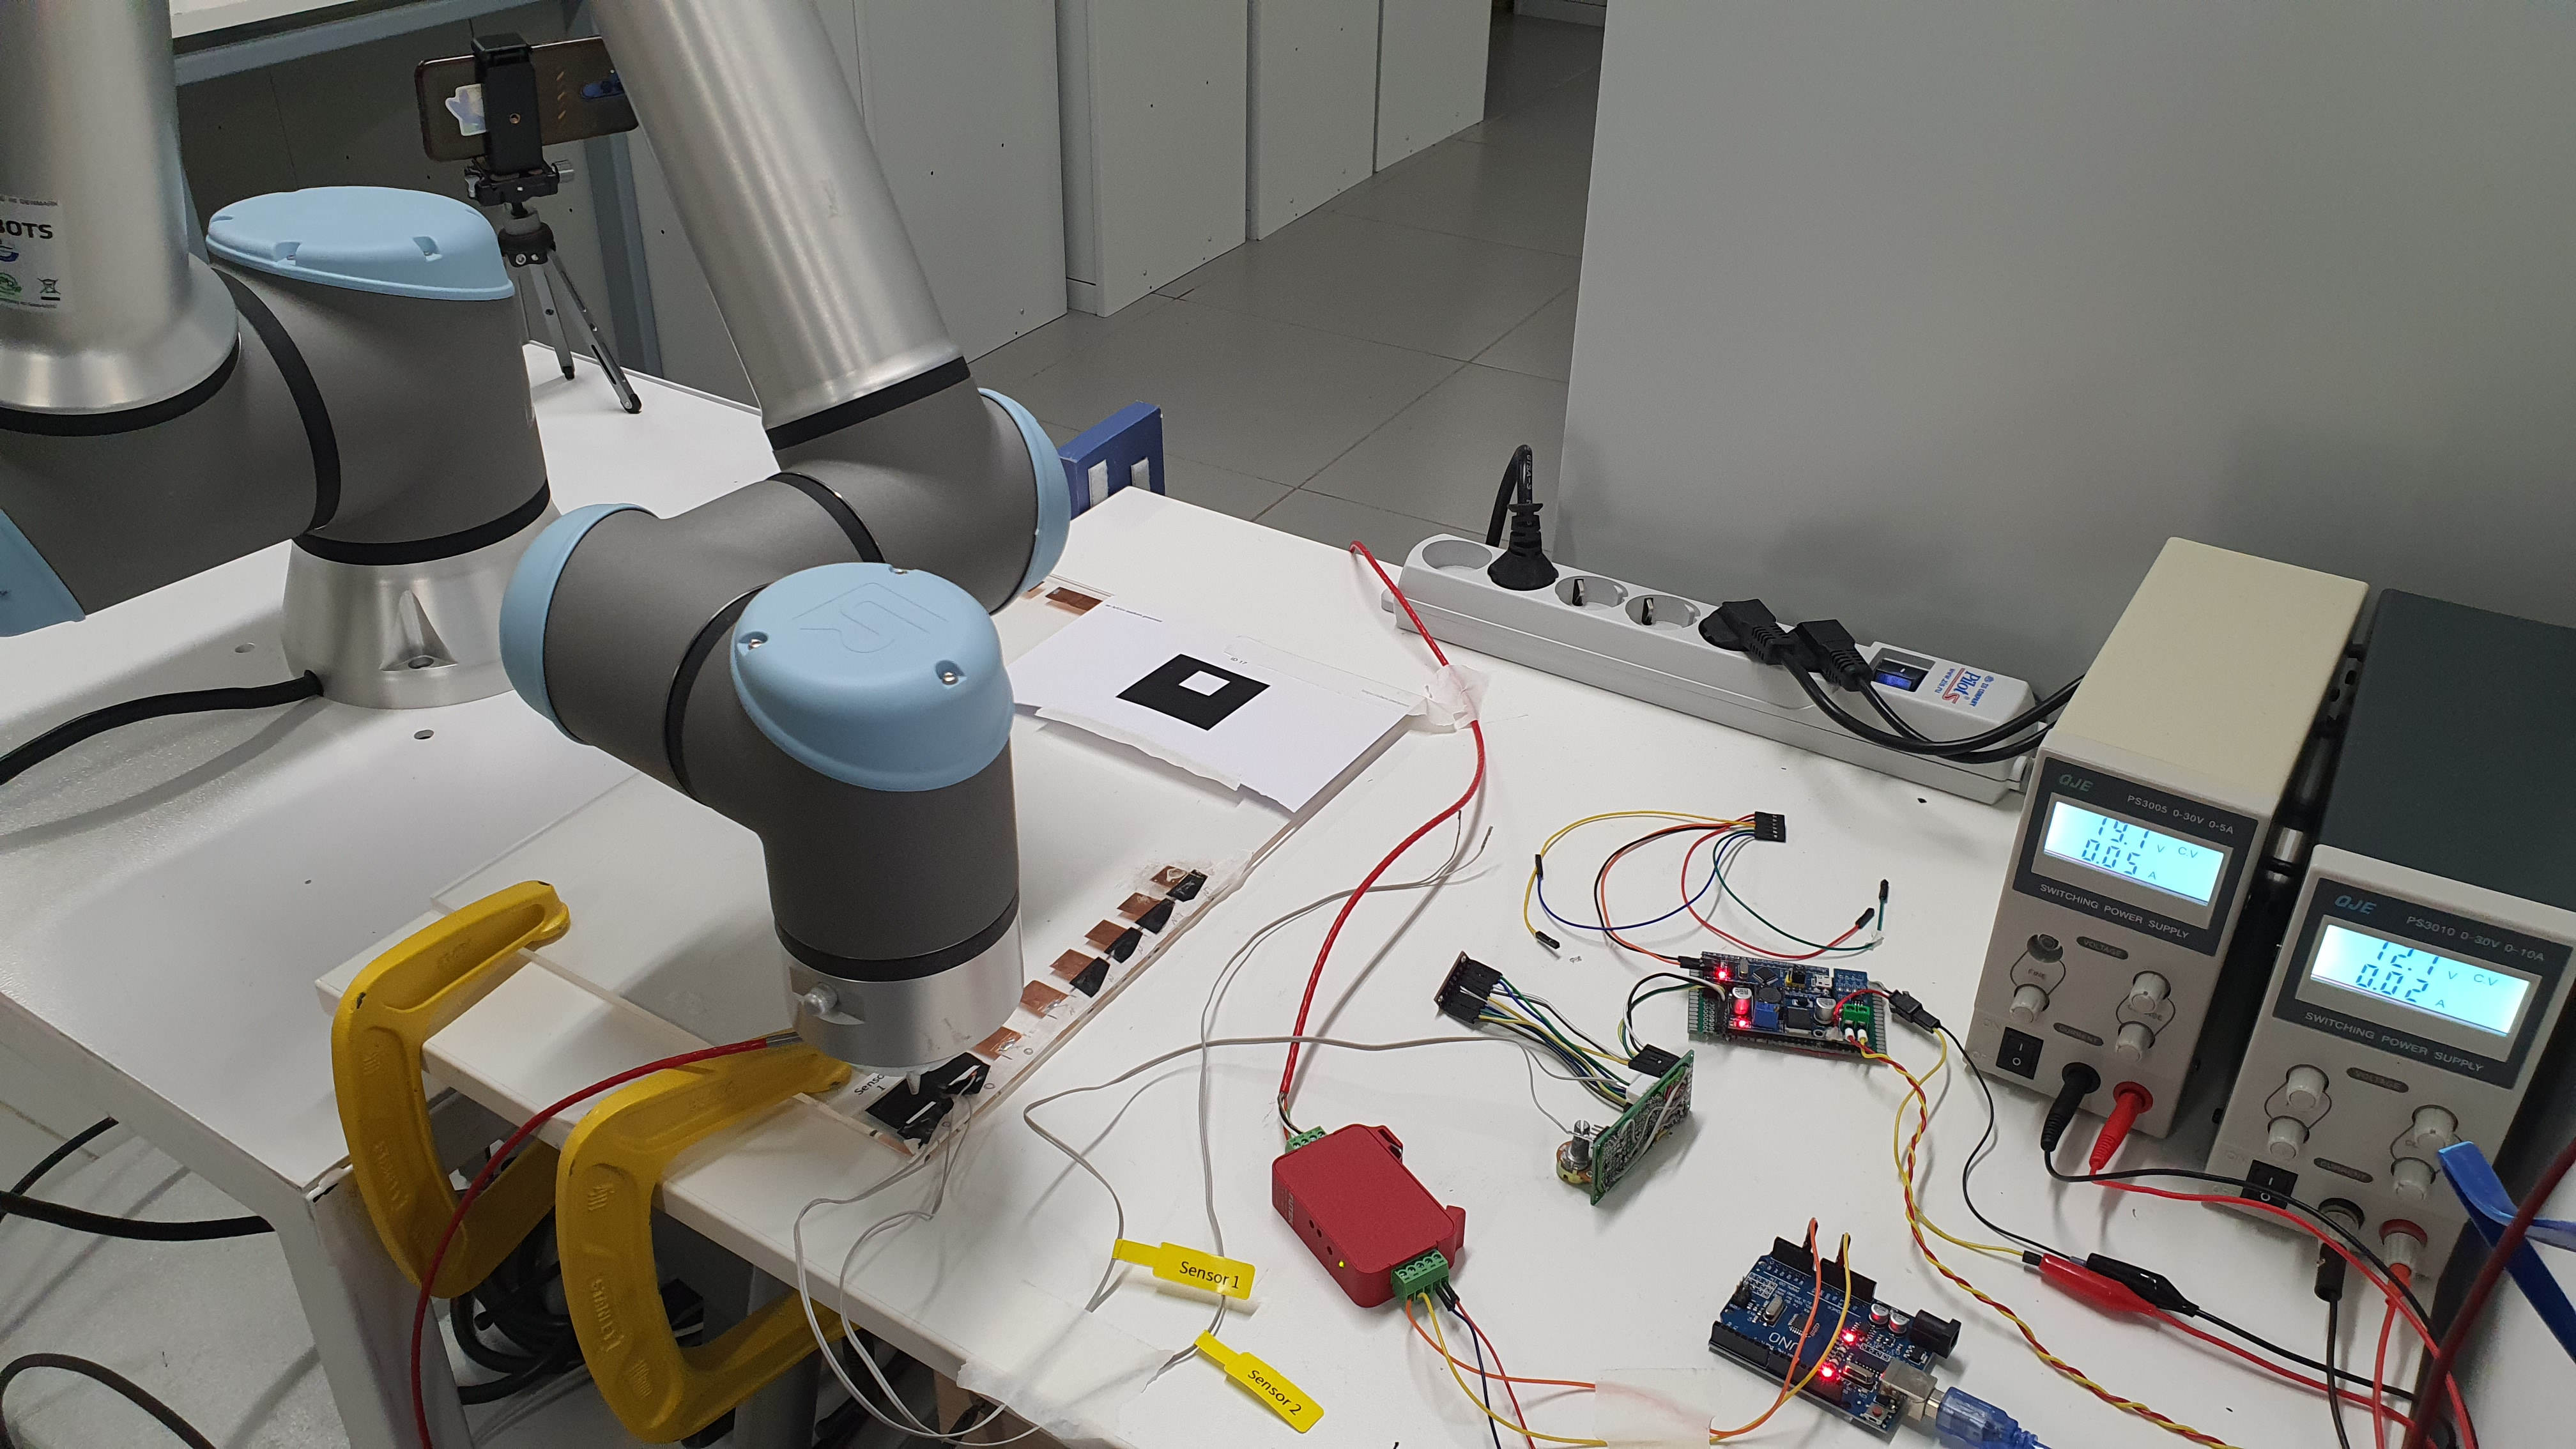
\includegraphics[height=6cm,width=1\textwidth,keepaspectratio]{exp_stand1}};

        % Create scope with normalized axes
        \begin{scope}[
                x={($0.1*(image.south east)$)},
                y={($0.1*(image.north west)$)}]

            % Grid
            % \draw[lightgray,step=1] (image.south west) grid (image.north east);

            % % Axes' labels
            % \foreach \x in {0,1,...,10} { \node [below] at (\x,0) {\x}; }
            % \foreach \y in {0,1,...,10} { \node [left] at (0,\y) {\y};}

            % Labels
            % \node[circle,fill=green] at (7.25,6.75){\small 2};

            \draw[latex-, very thick,green] (3.5,2.2) -- (2.5,1)
            node[below left,black,fill=white]{\small Velostat sensors};

            \draw[stealth-, very thick,green] (3.5,2.6) -- ++(-0.7,+0.5)
            node[left,black,fill=white]{\small Force sensor};

            \draw[stealth-, very thick,green] (6.5,3) -- (7,6)
            node[above right,black,fill=white]{\small Self made PCB};

            \draw[stealth-, very thick,green] (7.2,1.5) -- (8,5)
            node[above right,black,fill=white]{\small Arduino};

            \draw[stealth-, very thick,green] (2.5,9.5) -- (4,9.5)
            node[right,black,fill=white]{\small Camera};

            \draw[very thick,green] (0.5,2.5) rectangle (4.2,9)
            node[below left,black,fill=green]{\small UR5e};

            \draw[latex-, very thick,green] (4.5,7.2) edge (5.5,7.5)
            (4.8,5.3) -- (5.5,7.5)
            node[above,black,fill=white]{\small Aruco markers};
        \end{scope}

    \end{tikzpicture}
\end{center}
\end{frame}


\begin{frame}[t]{Force transducer design}
    \framesubtitle{Experimental Setup: Hardware, aruco markers}
    \vspace{-15pt}
    \begin{figure}[H]
        \centering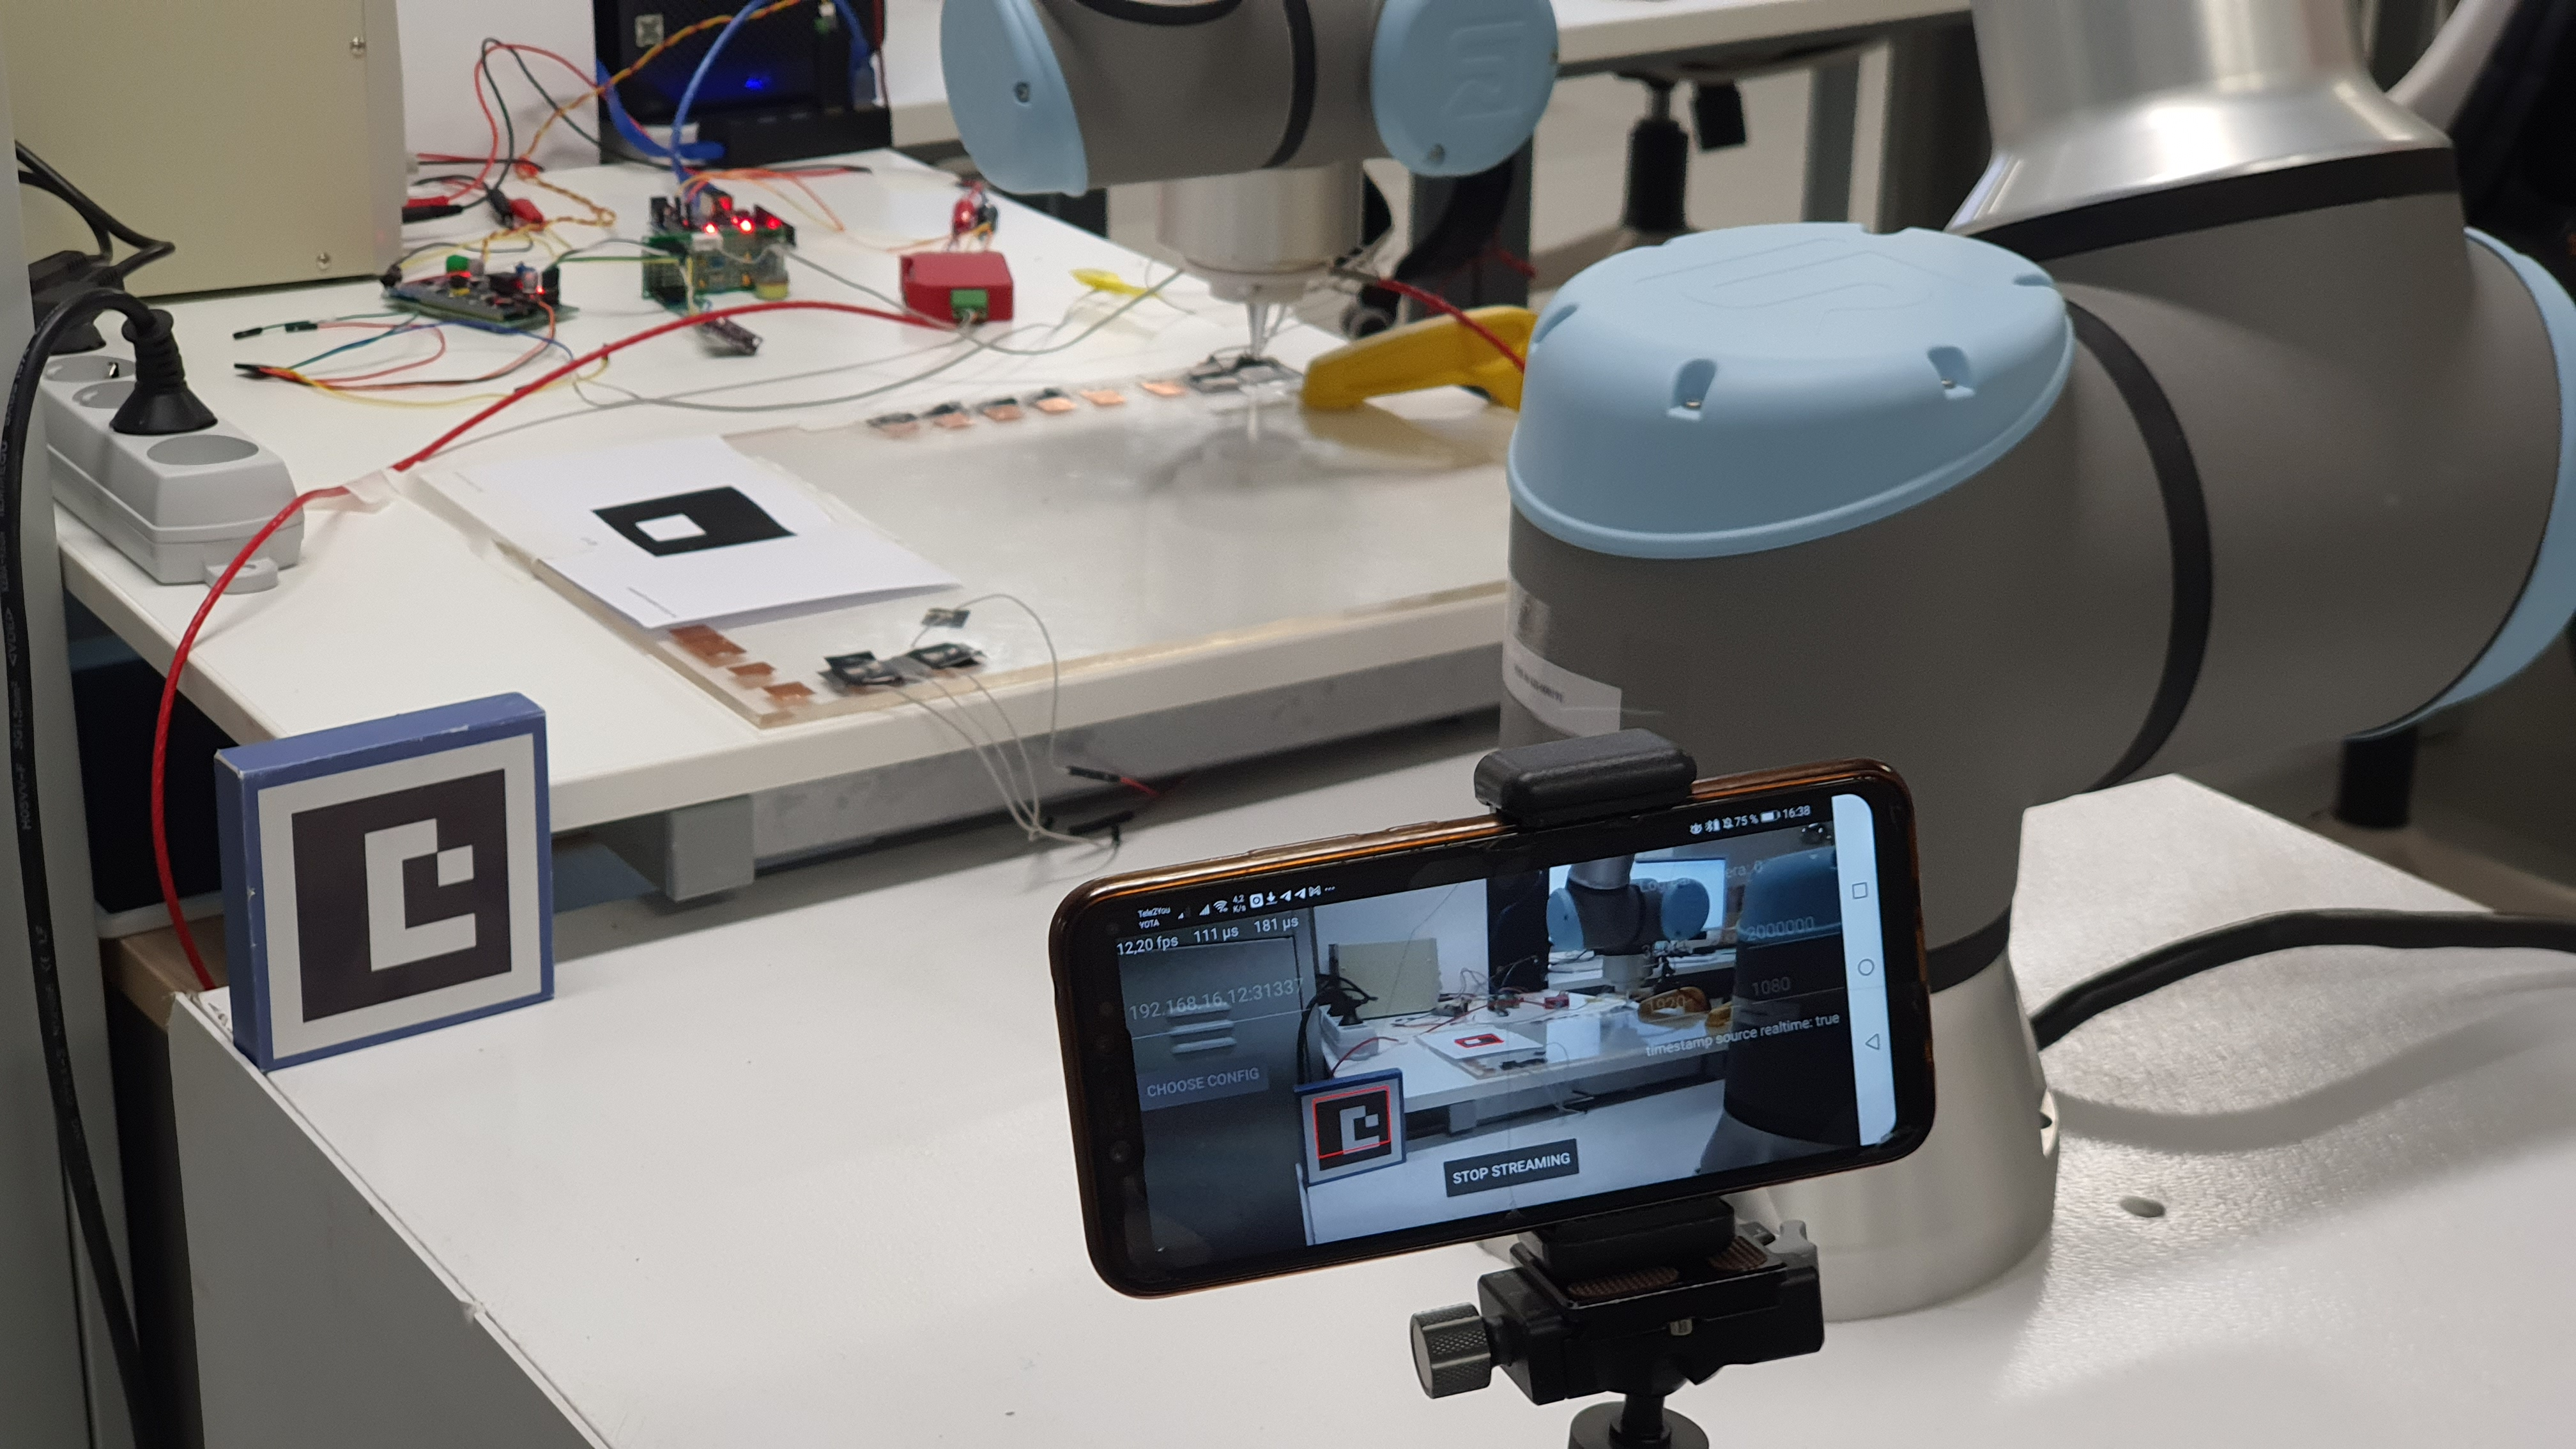
\includegraphics[height=6cm,width=1\textwidth,keepaspectratio]{exp_stand2}
        % \caption{caption_name}
        \label{fig:exp_stand2}
    \end{figure}
\end{frame}

\begin{frame}[t]{Force transducer design}
    \framesubtitle{Experimental Setup: Hardware, end-effector}
    \begin{figure}[H]
        \begin{subfigure}[t]{0.29\textwidth}
            \centering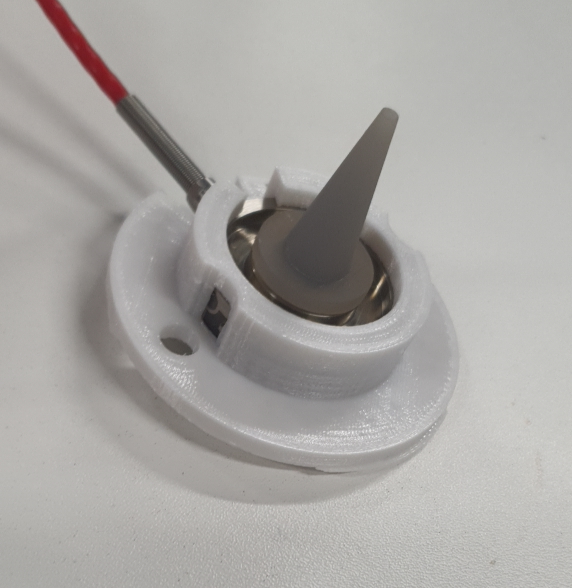
\includegraphics[width=0.99\textwidth]{point_load.JPG}\\
            \caption*{Point load: 2mm diameter}
            \label{fig:point_load}
        \end{subfigure}
        \begin{subfigure}[t]{0.29\textwidth}
            \centering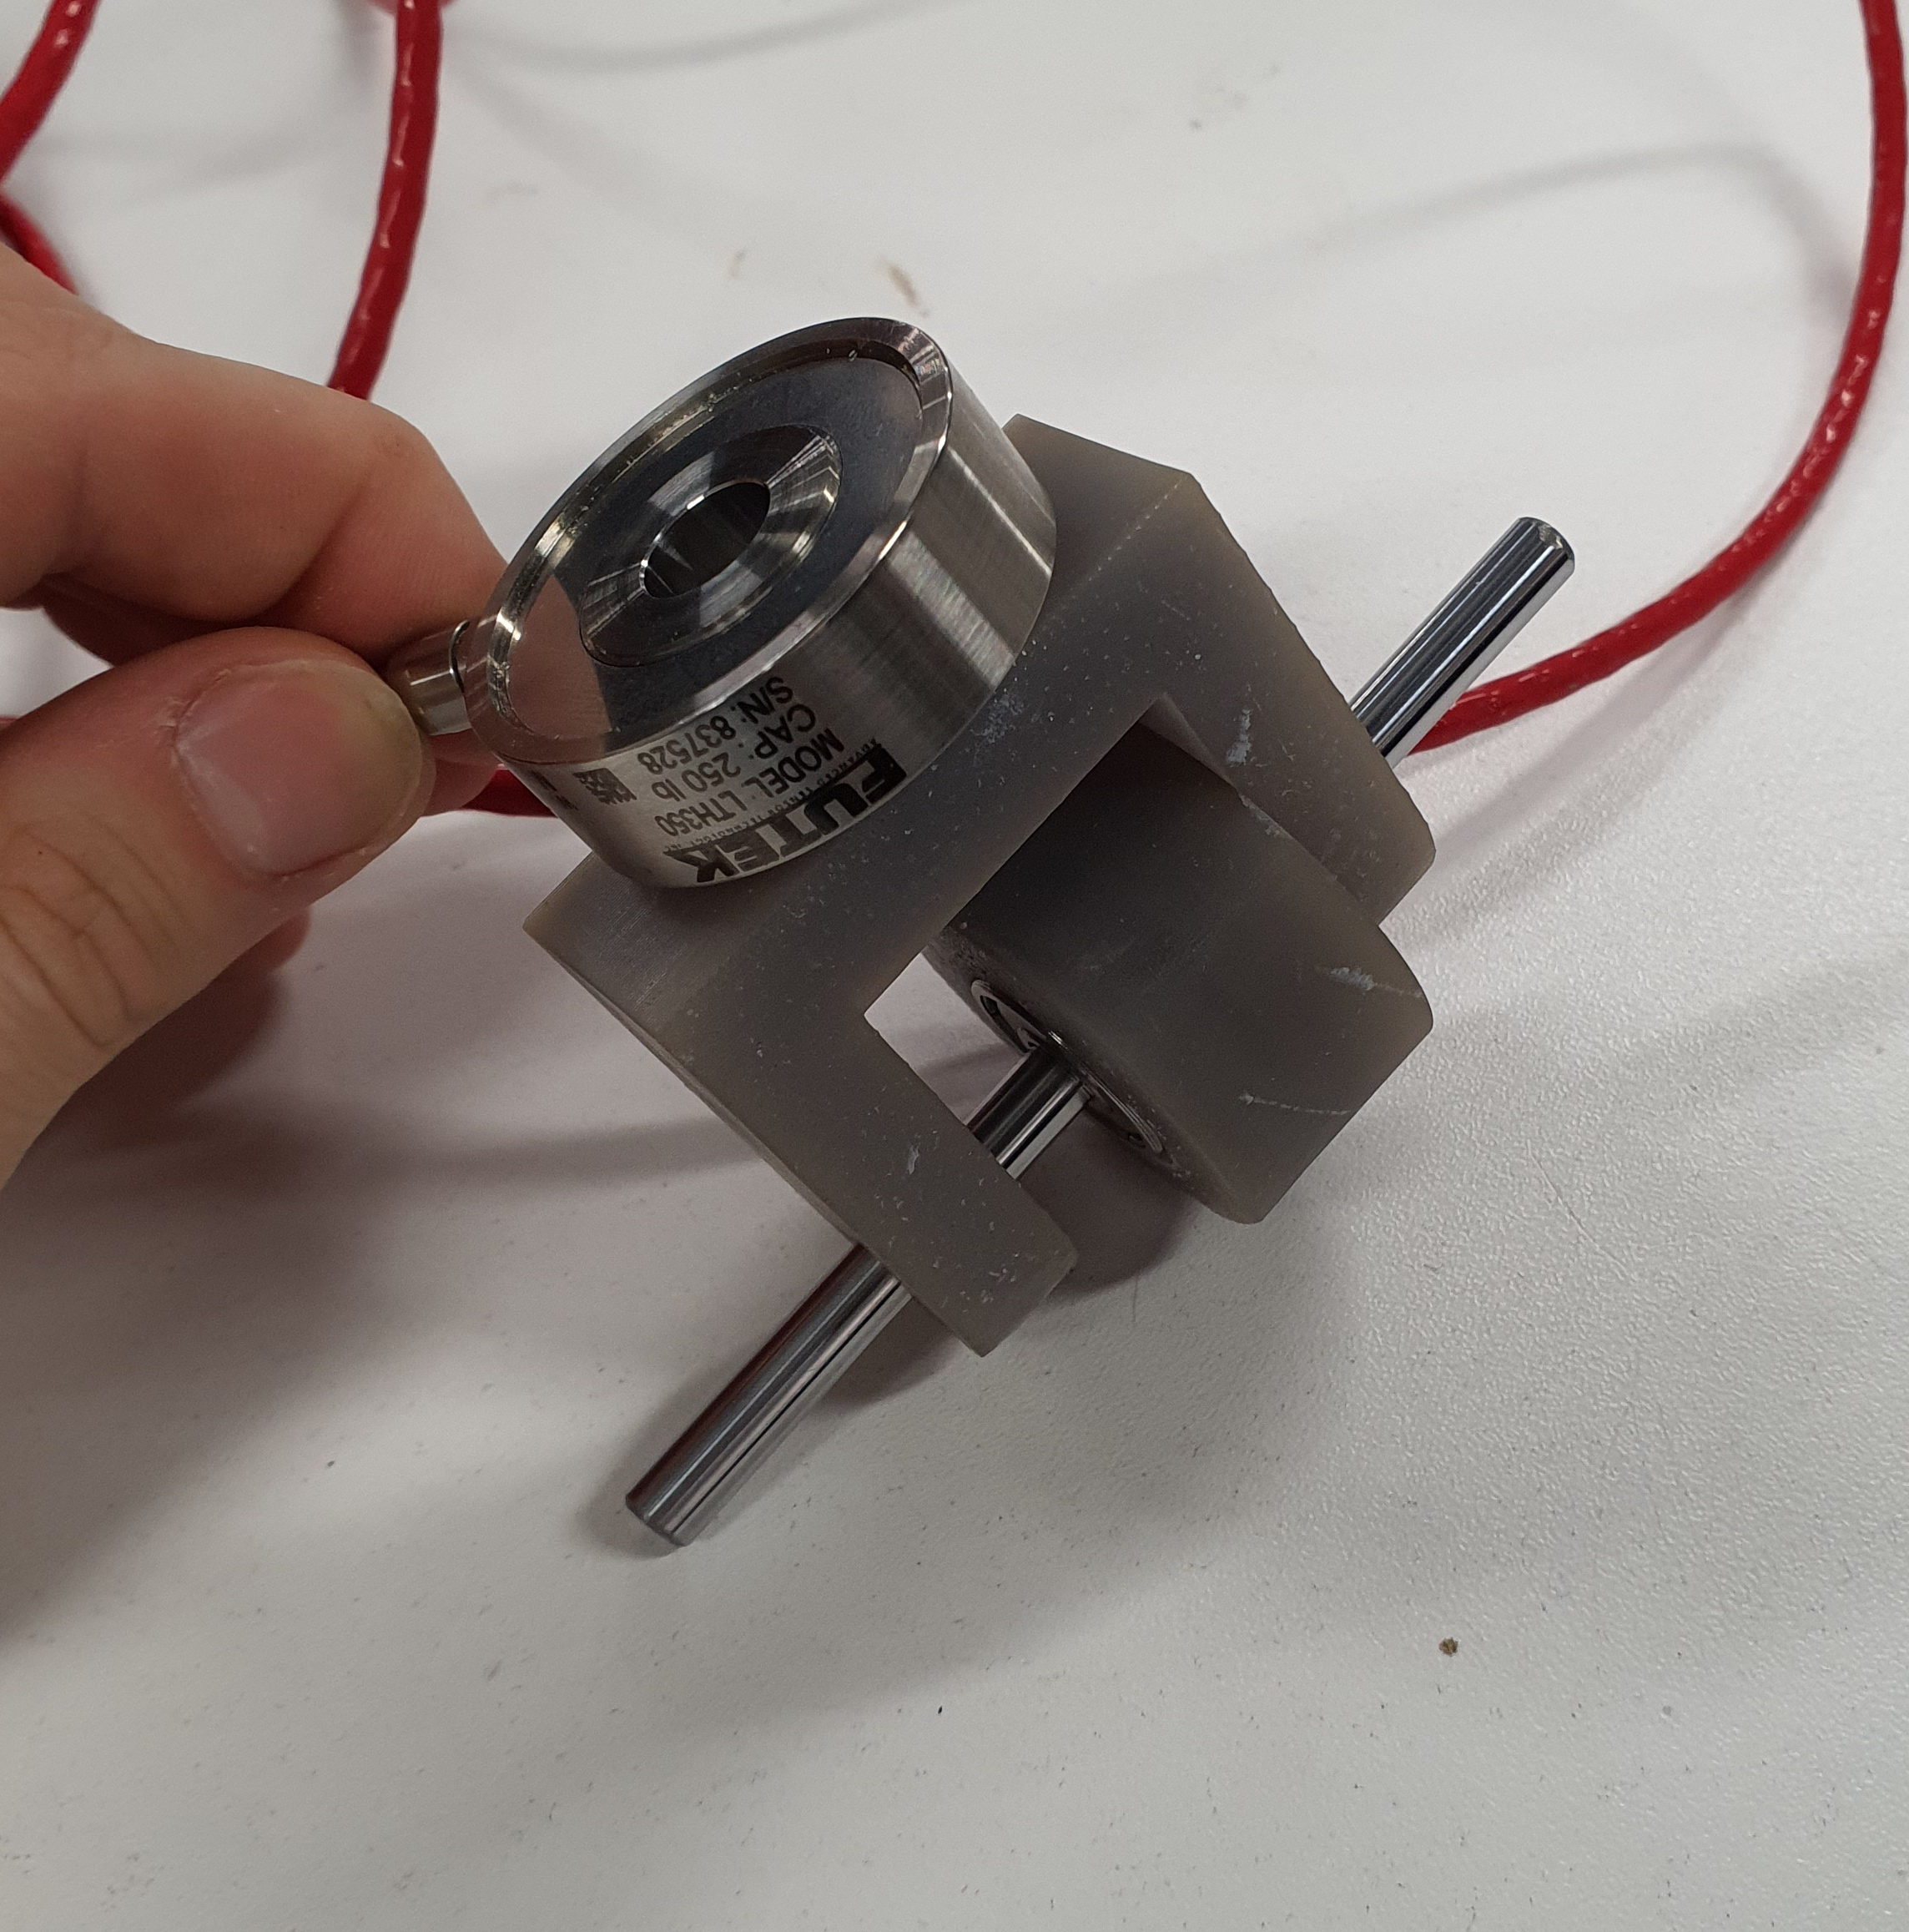
\includegraphics[width=0.99\textwidth]{rolling_load.JPG}\\
            \caption*{Rolling load}
            \label{fig:rolling_load}
        \end{subfigure}
        \begin{subfigure}[t]{0.29\textwidth}
            \centering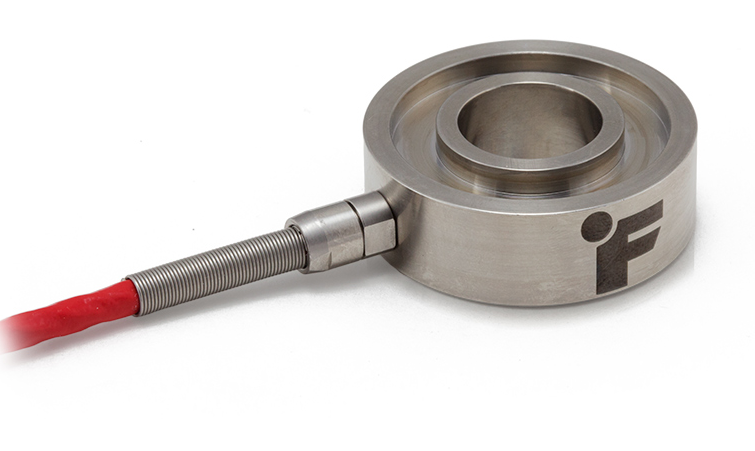
\includegraphics[width=0.99\textwidth]{LTH350-DONUT-LOAD-CELL-1.png}\\
            \caption*{Futek LTH350}
            \label{fig:futek}
        \end{subfigure}
    \end{figure}
\end{frame}

\begin{frame}[t]{Experiment Design}
    \framesubtitle{Experimental Setup: Hardware, video}
    \vspace{-15pt}
    \begin{figure}[H]
        \href{run:./videos/exp_stand_video.mp4}{
            \centering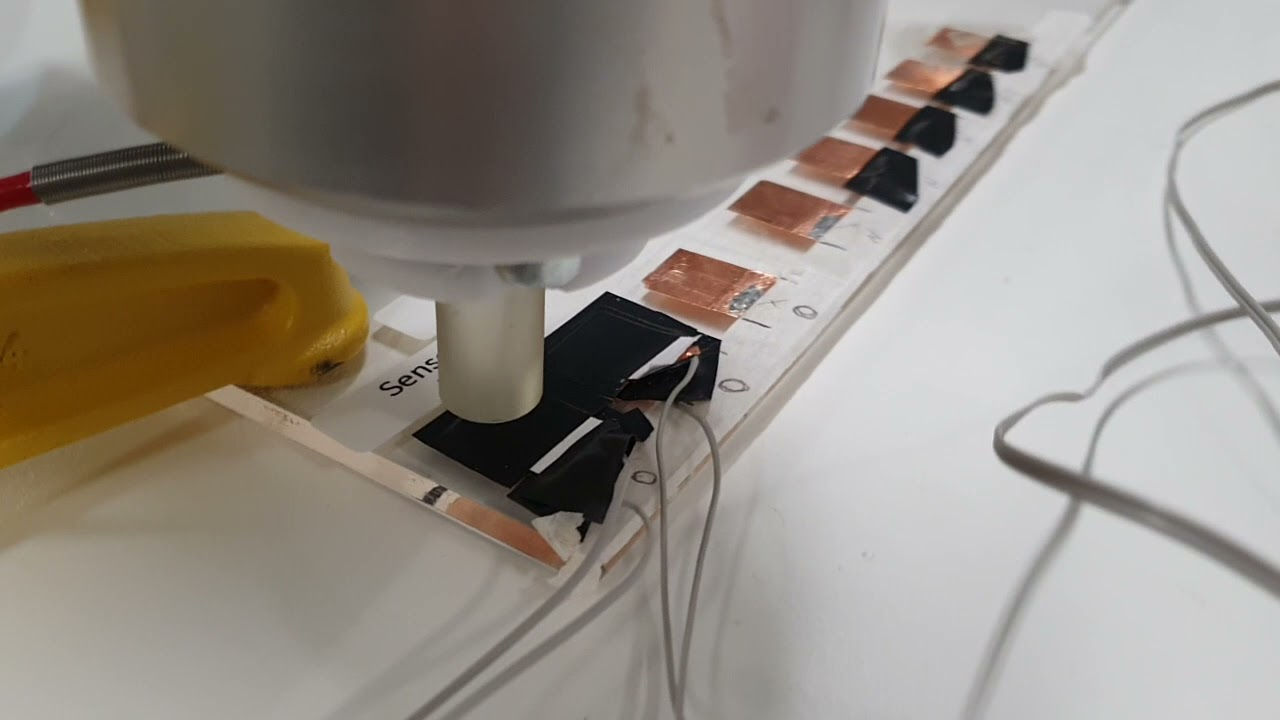
\includegraphics[height=6cm,width=1\textwidth,keepaspectratio]{exp_stand_video_preview.jpg}}
        % \caption{caption_name}
    \end{figure}
\end{frame}


\begin{frame}[t]{Force transducer design}
    \framesubtitle{Experiments}
    \vspace{-15pt}
    \begin{columns}[T,onlytextwidth]
        \begin{column}{0.6\textwidth}
            {\large
                \begin{enumerate}
                    \item \textbf{Static experiment}. The goal is to identify the coefficients for the transducer model.
                    \item\textbf{ Dynamic experiment}. 
                    \begin{itemize}
                        \item We are representing a transducer as a $4\times4$ matrix. We touch with the same pressure using five different end-effectors (area starting from 2mm till 15mm).
                        \item We are using 1st and last end-effector. We touch with different forces (5, 10, 20, 30, 40 H).
                    \end{itemize}
                \end{enumerate}
            }
        \end{column}
        \begin{column}{0.39\textwidth}
            \vspace{-0.5cm}
            \begin{figure}[H]
                \centering
                \begin{tikzpicture}
            
                    % Include the image in a node
                    \node [
                        above right,
                        inner sep=0] (image) at (0,0) {\centering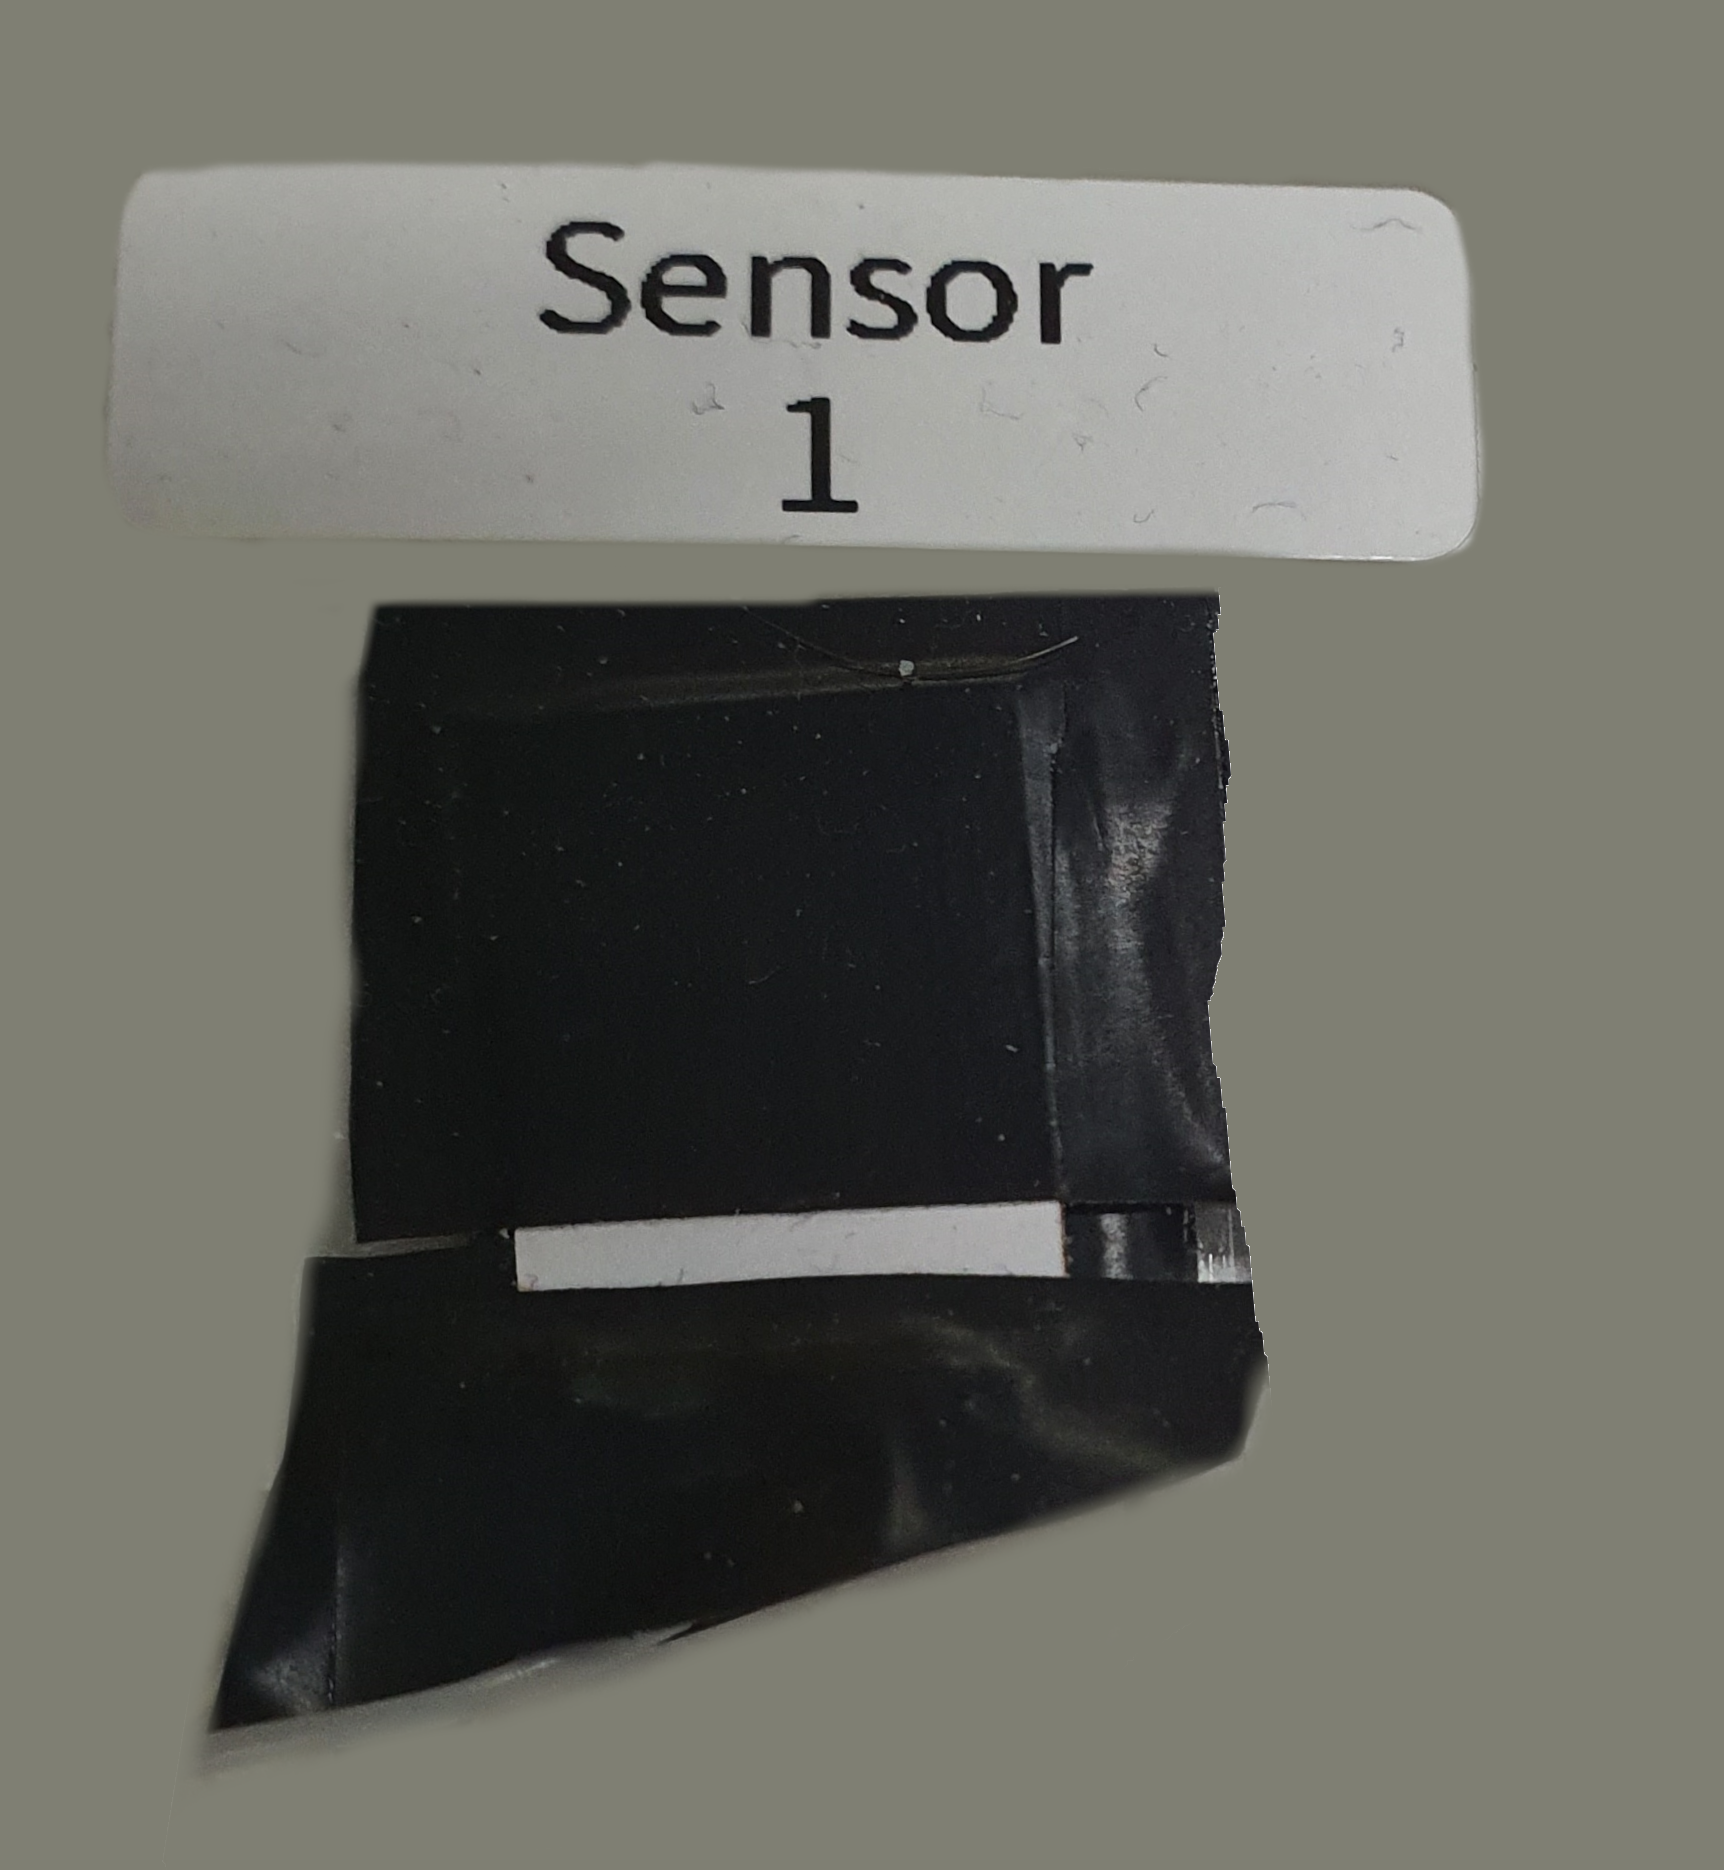
\includegraphics[height=5cm,width=1\textwidth,keepaspectratio]{sensors_grid.png}};
            
                    % Create scope with normalized axes
                    \begin{scope}[
                            x={($0.1*(image.south east)$)},
                            y={($0.1*(image.north west)$)}]
            
                        % Grid
                        % \draw[lightgray,step=1] (image.south west) grid (image.north east);
            
                        % % Axes' labels
                        % \foreach \x in {0,1,...,10} { \node [below] at (\x,0) {\x}; }
                        % \foreach \y in {0,1,...,10} { \node [left] at (0,\y) {\y};}
            
                        % Labels
                        % Simple brace
                        \draw [green, very thick,
                            decorate, 
                            decoration = {brace,
                                raise=5pt,
                                amplitude=5pt,
                                aspect=0.5}] (6,3.7) --  (3,3.7)
                        node[pos=0.5,below=10pt,green]{$15\ mm$};

                        \draw [green, very thick,
                        decorate, 
                        decoration = {brace, mirror,
                            raise=5pt,
                            amplitude=5pt,
                            aspect=0.5}] (6,3.6) --  (6,6.4)
                    node[pos=0.5,right=10pt,green]{$15\ mm$};

                    \draw[green,step=1,xshift=34, yshift=43]  (0.5,0.5) grid +(3,3);

                        \node[circle,fill=green,scale=0.4] at (3.3,6.27){\small 1};
                        \node[circle,fill=green,scale=0.4] at (5.92,3.7){\small 16};
            
                        % \draw[latex-, very thick,green] (3.5,2.2) -- (2.5,1)
                        % node[below left,black,fill=white]{\small Velostat sensors};
            
                        % \draw[stealth-, very thick,green] (3.5,2.6) -- ++(-0.7,+0.5)
                        % node[left,black,fill=white]{\small Force sensor};
            
                        % \draw[stealth-, very thick,green] (6.5,3) -- (7,6)
                        % node[above right,black,fill=white]{\small Self made PCB};
            
                        % \draw[stealth-, very thick,green] (7.2,1.5) -- (8,5)
                        % node[above right,black,fill=white]{\small Arduino};
            
                        % \draw[stealth-, very thick,green] (2.5,9.5) -- (4,9.5)
                        % node[right,black,fill=white]{\small Camera};
            
                        % \draw[very thick,green] (0.5,2.5) rectangle (4.2,9)
                        % node[below left,black,fill=green]{\small UR5e};
            
                        % \draw[latex-, very thick,green] (4.5,7.2) edge (5.5,7.5)
                        % (4.8,5.3) -- (5.5,7.5)
                        % node[above,black,fill=white]{\small Aruco markers};
                    \end{scope}

                \end{tikzpicture}
                \caption*{Sensor representation \\ as 4x4 grid}
                \label{fig:file_name}
            \end{figure}
        \end{column}
    \end{columns}

\end{frame}

\begin{frame}[t]{Force transducer design}
    \framesubtitle{Result: static experiment}
    \vspace{-0.5cm}
    \begin{columns}[T,onlytextwidth]
        \begin{column}{0.52\textwidth}
            \begin{eqnarray*}
                V_{out} = V_0 + p[k_p + k_e(1-e^\frac{-(t-t_0)}{\tau_{res}})](1-e^{-\frac{A}{p}}) \\
                k_p = A_1e^{-A_2p}; \tau_{res} = B_0 + B_1e^{-\frac{p}{B_2}}
            \end{eqnarray*}
            Where $V_0$ -- initial voltage, $p,\ A_i,\ B_i,\ \tau_{res},\ k_i$ are constants, $t$ -- current time, $t_0$ -- the time when the pressure appeared.
        \end{column}
        \begin{column}{0.45\textwidth}
            \vspace{-15pt}
            \begin{figure}[H]
                \centering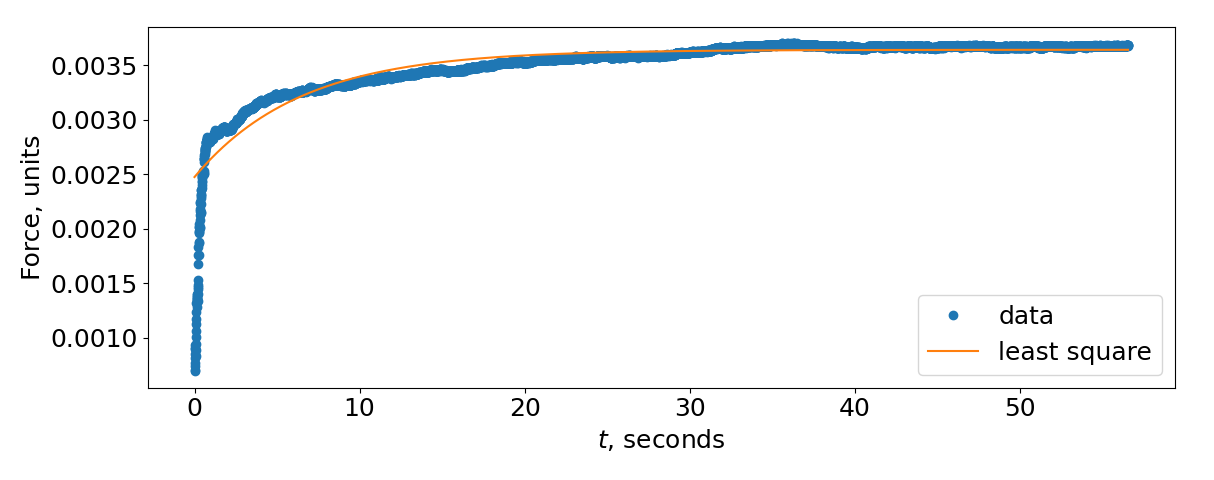
\includegraphics[height=2.8cm,width=1\textwidth,keepaspectratio]{least_square_model.png}
                \label{fig:least_square_model.png}
            \end{figure}
        \end{column}
    \end{columns}
    \vspace{-11pt}
    \begin{figure}[H]
        \centering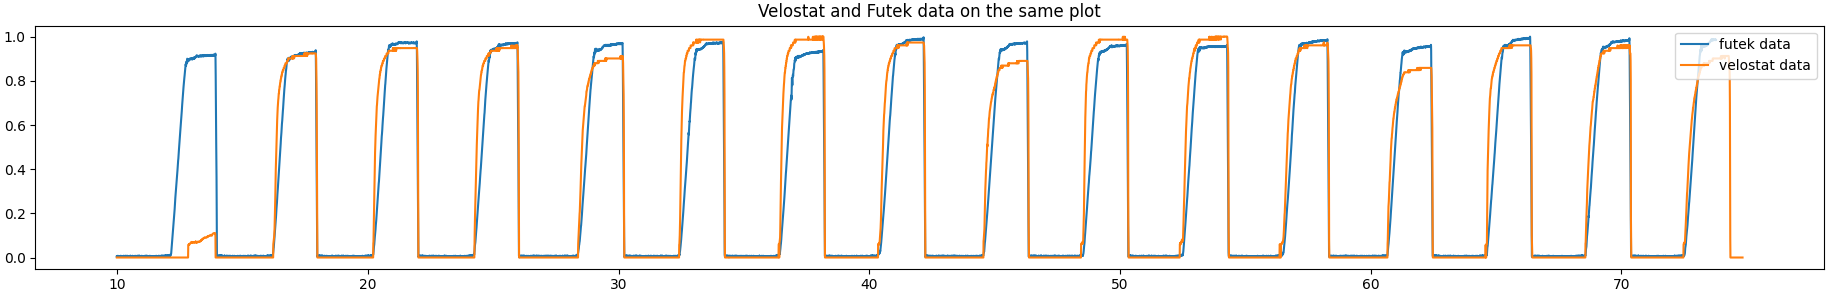
\includegraphics[height=3cm,width=1\textwidth,keepaspectratio]{pikes.png}
        \caption*{ Normalized force data from sensor and transducer}
        \label{fig:pikes.png}
    \end{figure}
\end{frame}

\begin{frame}[t]{Force transducer design}
    \framesubtitle{Result: dynamic experiment}
    \vspace{-15pt}
    \begin{figure}[H]
        \begin{subfigure}{0.49\textwidth}
            \centering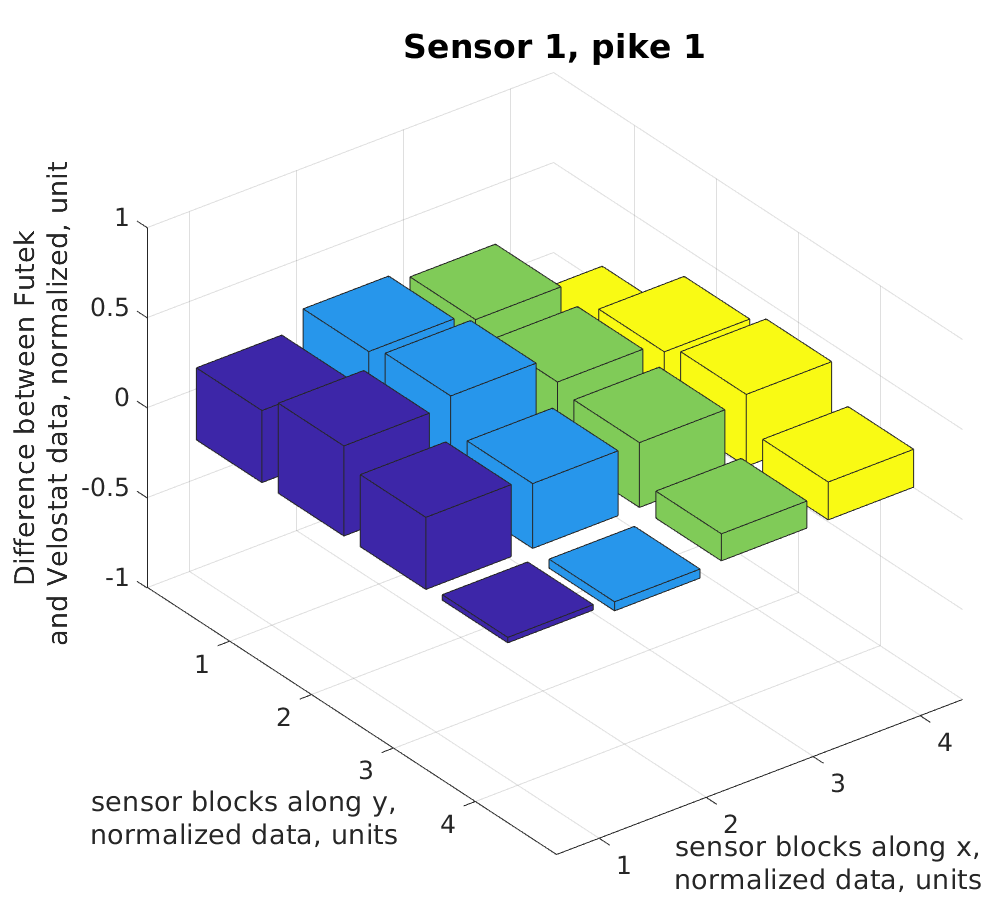
\includegraphics[height=5cm,width=1\textwidth,keepaspectratio]{sens1_pike1.png}
            \caption*{2mm end-effector diam}
            \label{fig:sens1_pike1}
        \end{subfigure}
        \begin{subfigure}{0.49\textwidth}
            \centering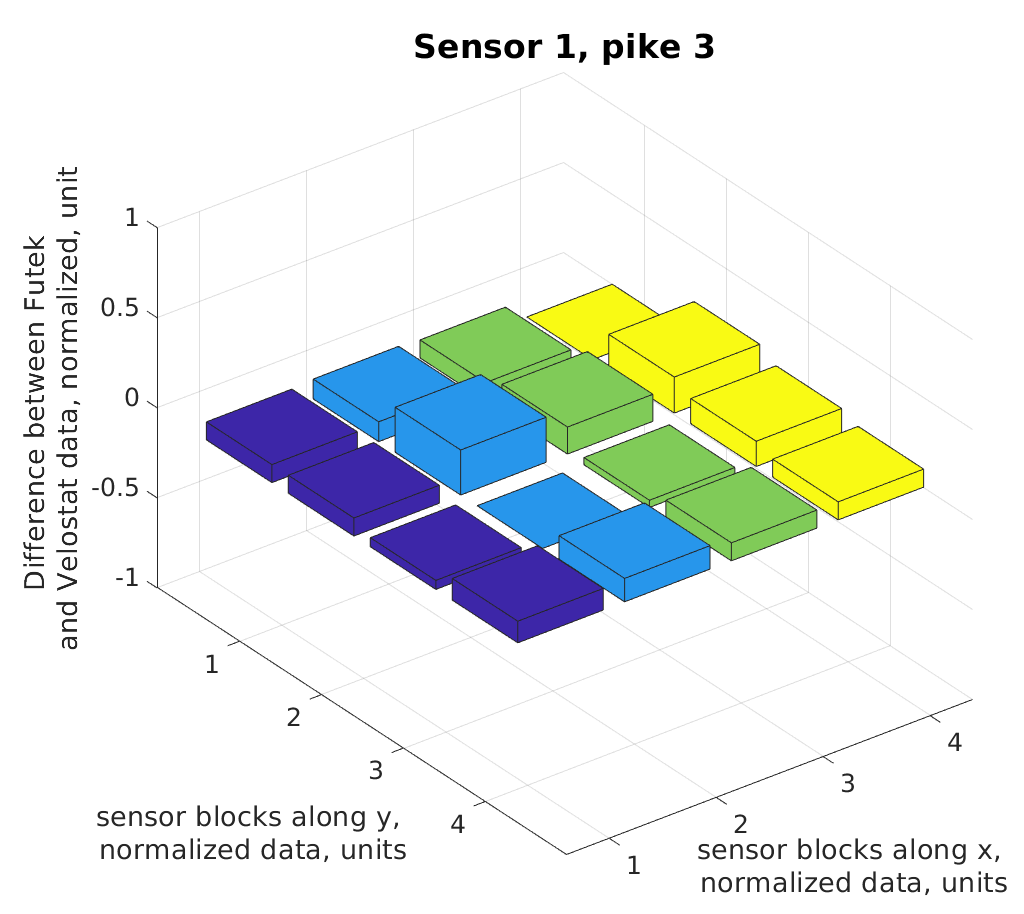
\includegraphics[height=5cm,width=1\textwidth,keepaspectratio]{sens1_pike3.png}
            \caption*{8mm end-effector diam}
            \label{fig:sens1_pike3}
        \end{subfigure}
    \end{figure}
\end{frame}

\begin{frame}[t]{Force transducer design}
    \framesubtitle{Summary}
    \vspace{-15pt}
    {\Large
        \begin{enumerate}
            \item Static experiment: transducers coefficients were identified.
            \item Dynamic experiment: a transducer can be represented as one body, when pressure area is higher than 50\% of the sensor area.
        \end{enumerate}
    }
\end{frame}

\begin{frame}[t]{Terrain classification}
    \framesubtitle{}
    \only<1-2>{\LARGE\begin{block}{Question}
            How to define the terrain type during the movement on such terrain?
        \end{block}}
    \only<2>{\LARGE\begin{alertblock}{Answer}
            \centering Solving terrain classification problem using Machine learning
        \end{alertblock}}
\end{frame}

\begin{frame}[t]{Terrain classification}
    \framesubtitle{Experimental Setup}
    \vspace{-15pt}
    \begin{columns}[T,onlytextwidth]
        \begin{column}{0.49\textwidth}
            \begin{enumerate}
                \item Dynamixel MX28 -- 47 rev/min
                \item Velostat transducer -- 25 HZ freq.
                \item Experiment duration -- 120 sec
            \end{enumerate}
            \vspace{-0.3cm}
            \begin{figure}[H]
                \centering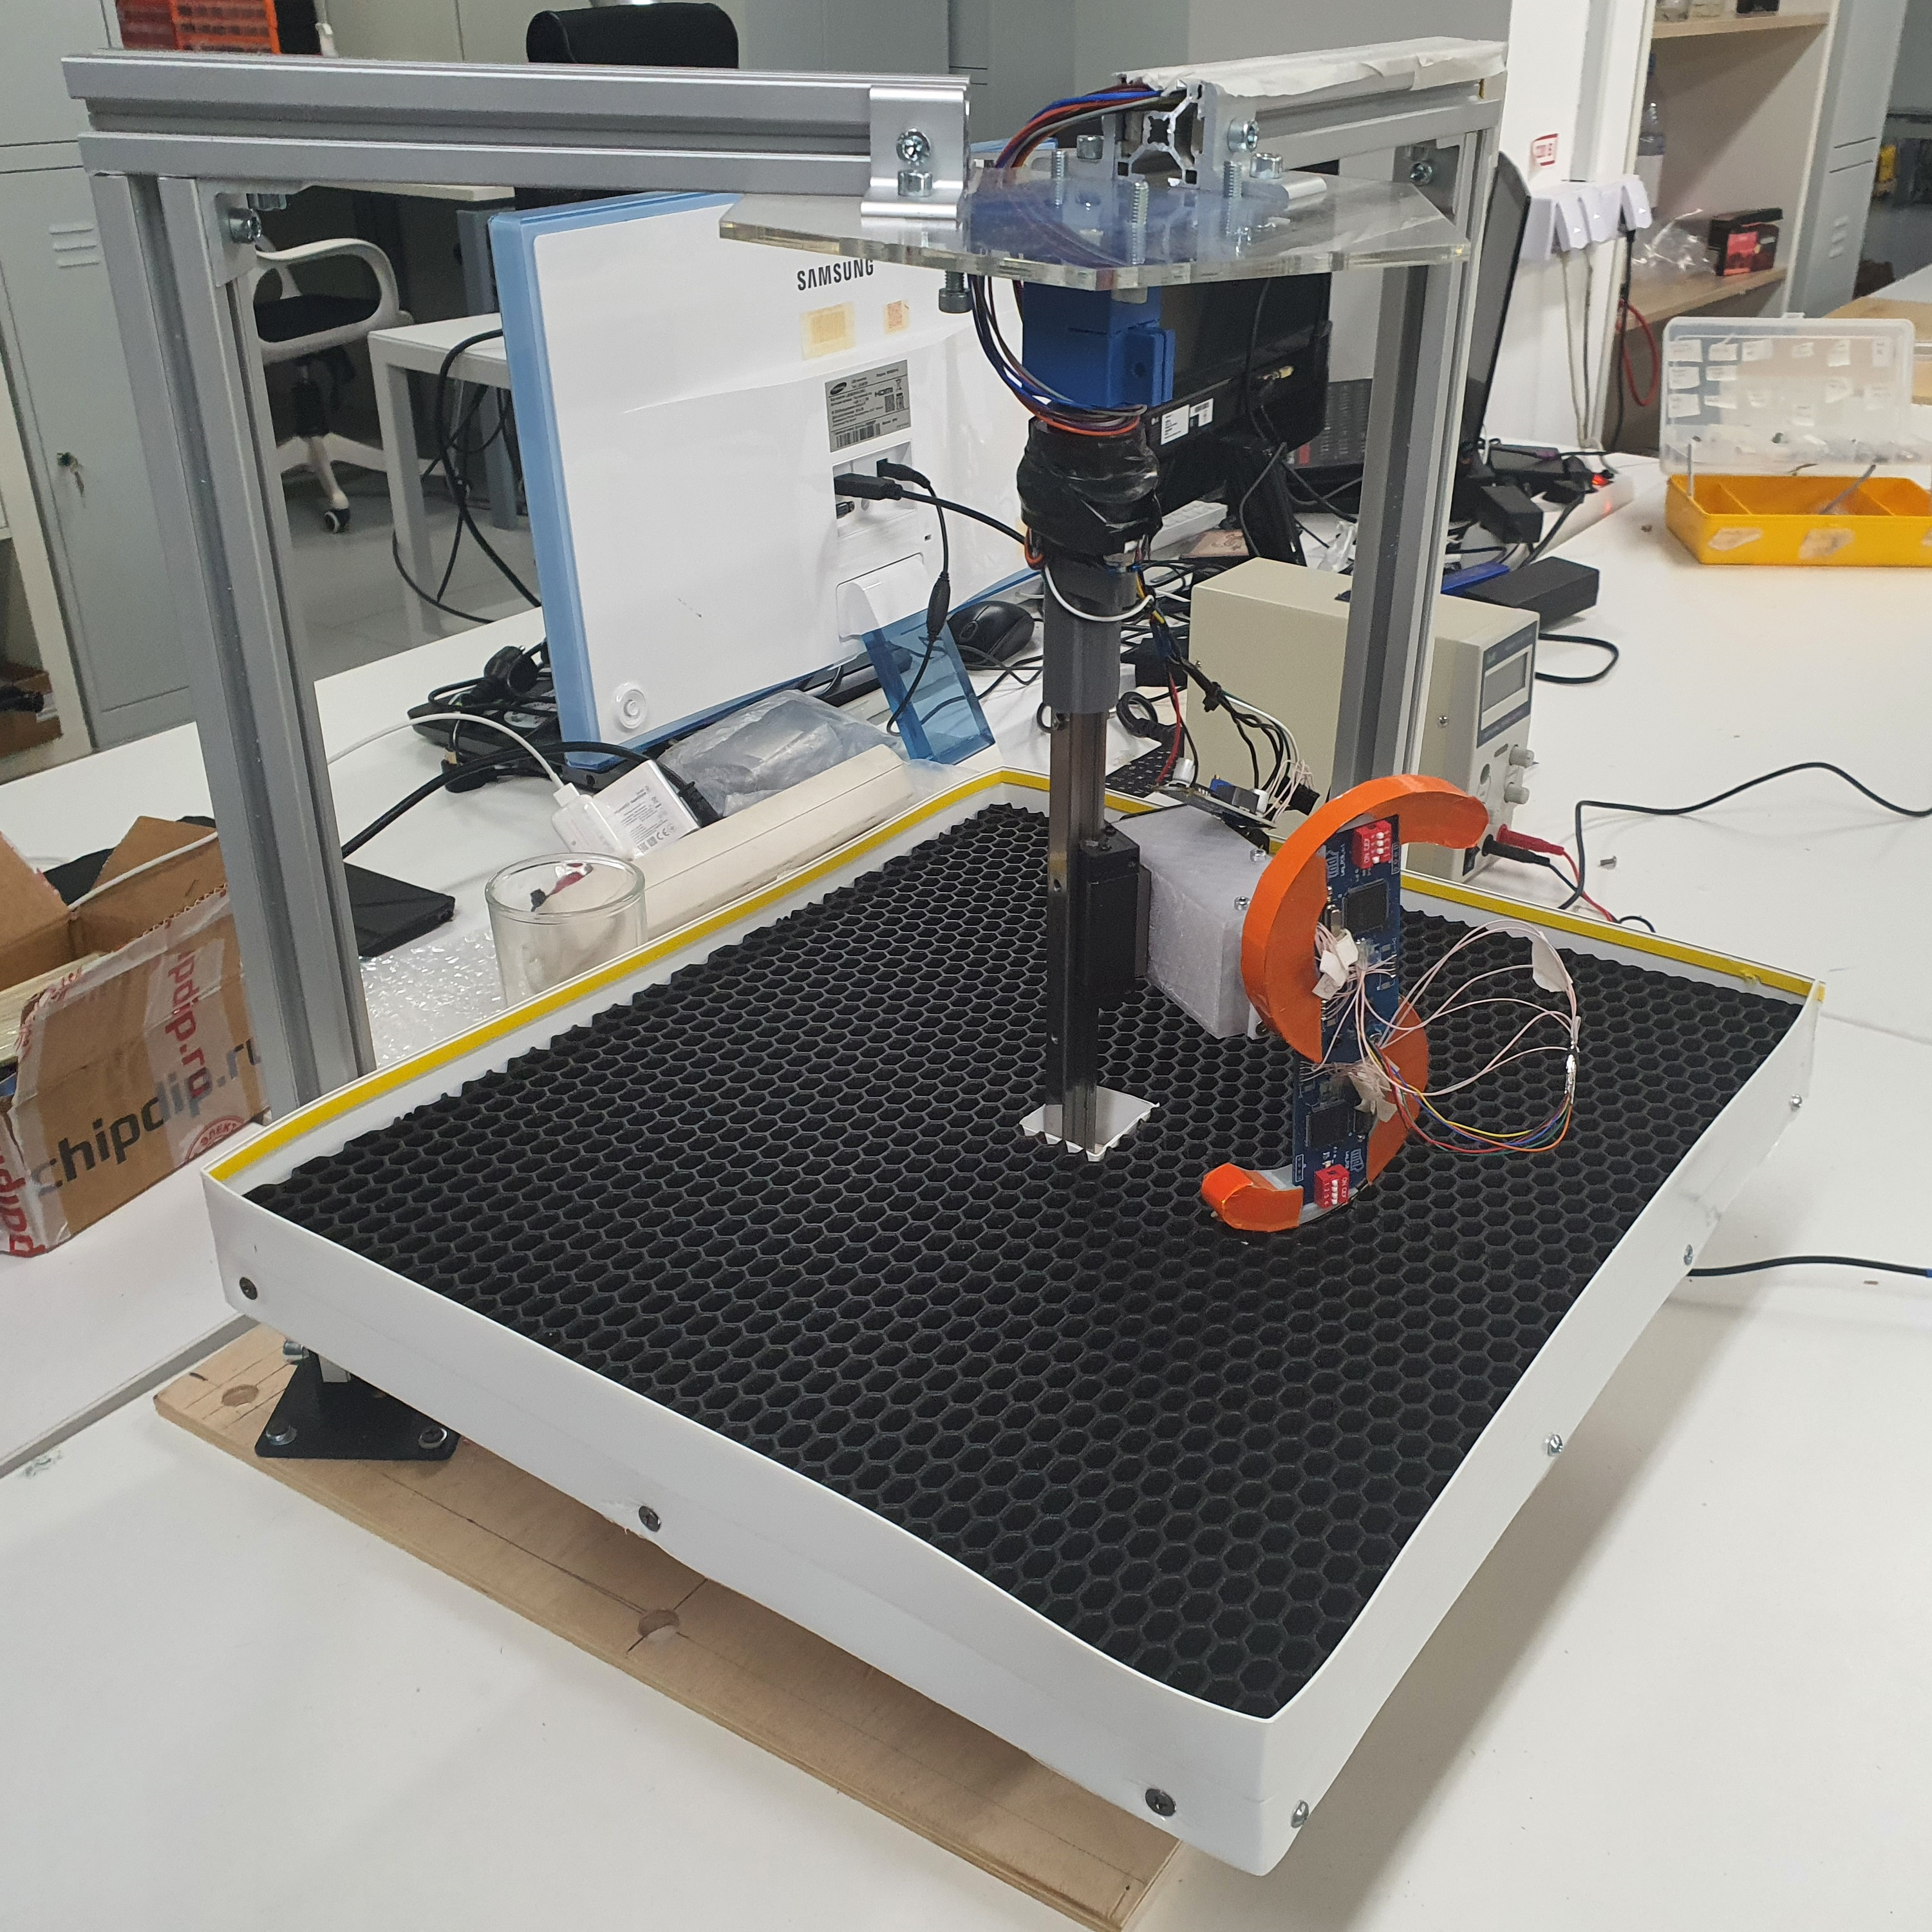
\includegraphics[height=4cm,width=1\textwidth,keepaspectratio]{s_shape_leg/s_leg_setup.JPG}
                % \caption{caption_name}
                \label{fig:s_shape_leg/}
            \end{figure}
        \end{column}
        \begin{column}{0.49\textwidth}
            \vspace{-0.5cm}
            \begin{figure}[H]
                \begin{subfigure}{\textwidth}
                    \centering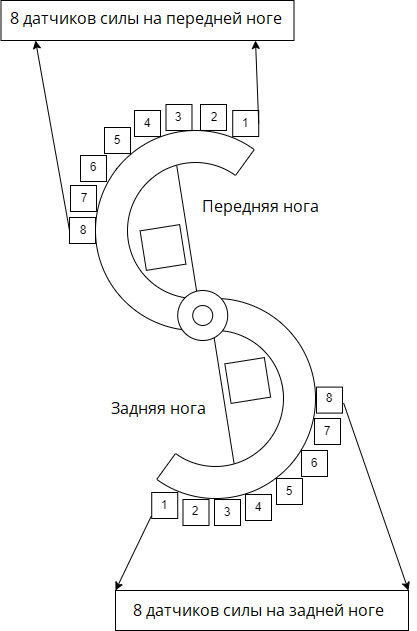
\includegraphics[height=6cm,width=1\textwidth,keepaspectratio]{s_shape_leg/leg_design.png}
                    % \caption{caption_name}
                \end{subfigure}
            \end{figure}
        \end{column}
    \end{columns}
\end{frame}


\begin{frame}[t]{Terrain classification}
    \framesubtitle{Experimental setup: terrain types, video}
    \vspace{-15pt}
    \begin{figure}[H]
        \begin{subfigure}{0.49\textwidth}
            \href{run:./videos/flat.gif}{\centering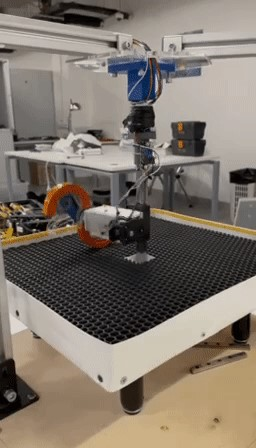
\includegraphics[height=6cm,width=1\textwidth,keepaspectratio]{s_shape_leg/flat.jpg}}
            % \caption*{2mm end-effector diam}    
        \end{subfigure}
        \hfill
        \begin{subfigure}{0.49\textwidth}
            \href{run:./videos/rock.gif}{\centering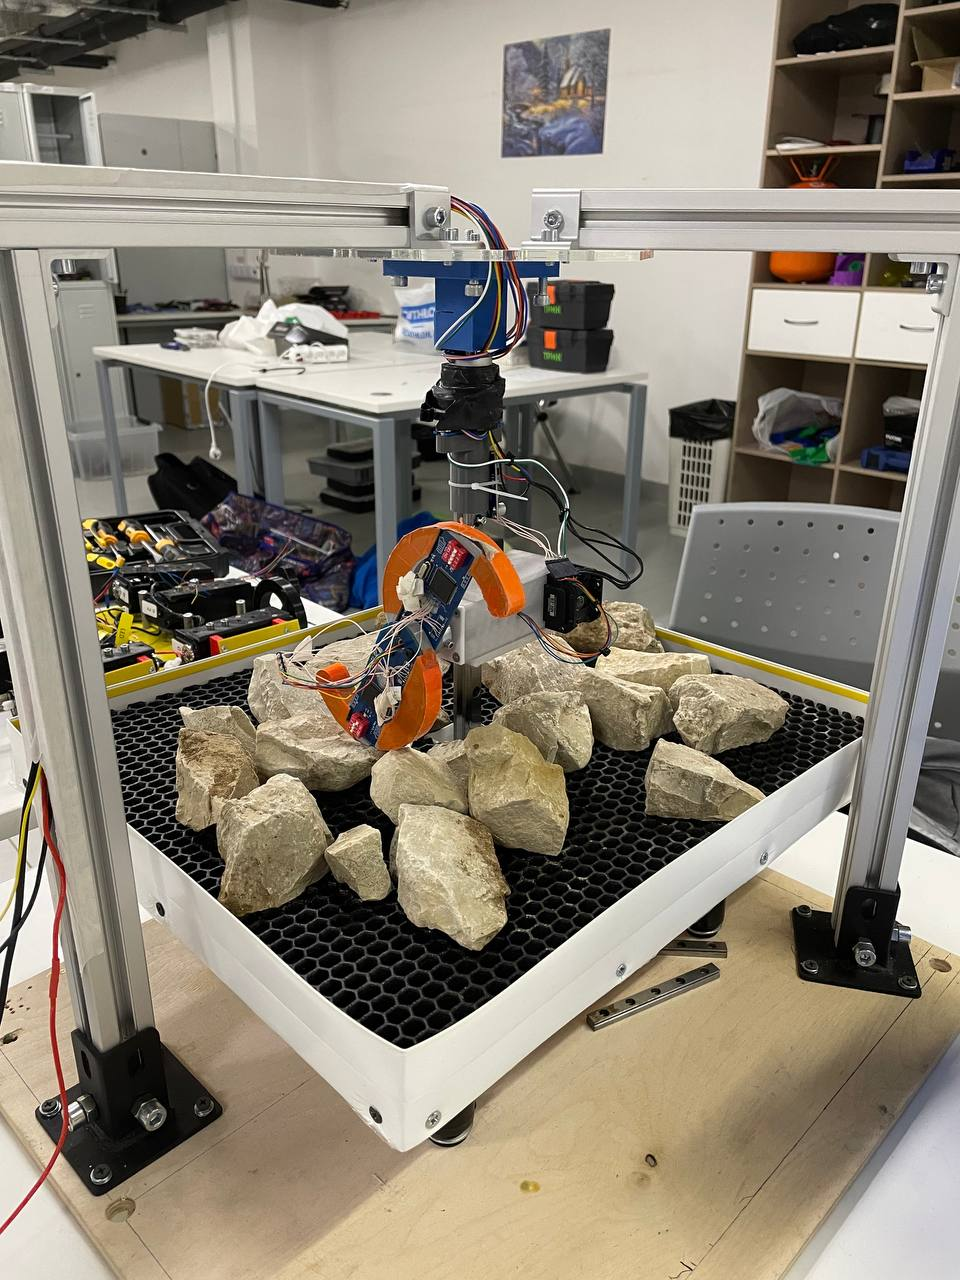
\includegraphics[height=6cm,width=1\textwidth,keepaspectratio]{s_shape_leg/view.jpg}}
            % \caption*{8mm end-effector diam}
        \end{subfigure}
    \end{figure}
\end{frame}

\begin{frame}[t]{Terrain classification}
\framesubtitle{Velostat transducer properties}
\Large
\begin{itemize}
    \item 'cause of high hysteresis and difficulties with calibration, we have to work with relative data.
\end{itemize}
    
\end{frame}

\begin{frame}[t]{Terrain classification}
    \framesubtitle{Obtained data from one experiment}
    \begin{columns}[T,onlytextwidth]
        \begin{column}{0.49\textwidth}
            \begin{figure}[H]
                \centering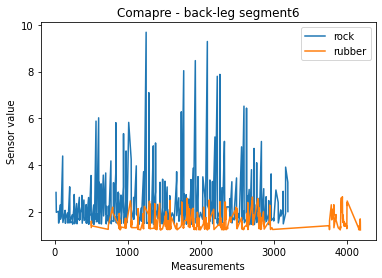
\includegraphics[height=5cm,width=1\textwidth,keepaspectratio]{s_shape_leg/segment6_compare.png}
            \end{figure}
        \end{column}
        \begin{column}{0.49\textwidth}
            \vspace{-2.4cm}
            \begin{figure}[H]
                \begin{subfigure}{0.99\textwidth}
                    \centering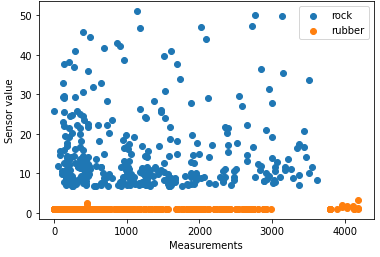
\includegraphics[height=3.8cm,width=1\textwidth,keepaspectratio]{s_shape_leg/segment8_compare_front.png}
                    % \caption*{2mm end-effector diam}    
                \end{subfigure}

                \begin{subfigure}{0.99\textwidth}
                    \centering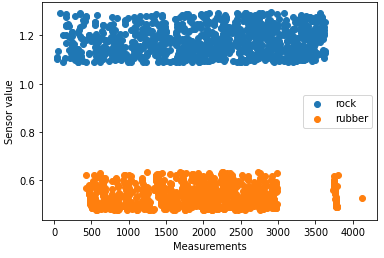
\includegraphics[height=3.8cm,width=1\textwidth,keepaspectratio]{s_shape_leg/segment6_compare_front.png}
                    % \caption*{8mm end-effector diam}
                \end{subfigure}
            \end{figure}
        \end{column}
    \end{columns}
\end{frame}

\begin{frame}[t]{Terrain classification}
    \framesubtitle{Summary}
    \Large
    \begin{itemize}
        \item Can distinct rubber and rock terrains
        \item Choose terrain classification parameters
              \begin{itemize}
                  \item RPM
                  \item Motor Torque
                  \item Acceleration from IMU
                  \item Force data which are represented as Sensor value\/segment, Peak amplitude, Average amplitude
              \end{itemize}
        \item Prove that force transducer is working
    \end{itemize}
\end{frame}

\begin{frame}[t]{Map creation based on tactile data}
    \framesubtitle{}
    \only<1-2>{\LARGE\begin{block}{Question}
            How to create a dense point cloud, using sparse data from legs?
        \end{block}}
    \only<2>{\LARGE\begin{alertblock}{Answer}
            \centering \textit{Take this data}, \textit{create a mesh} using concave hull Delaunay triangulation, \textit{sampling it} and return to the main algorithm
        \end{alertblock}}
\end{frame}

\begin{frame}[t]{Map creation based on tactile data}
    \framesubtitle{Experimental setup}
    \vspace{-15pt}
    \begin{figure}[H]
        \begin{subfigure}[t]{0.49\textwidth}
            \centering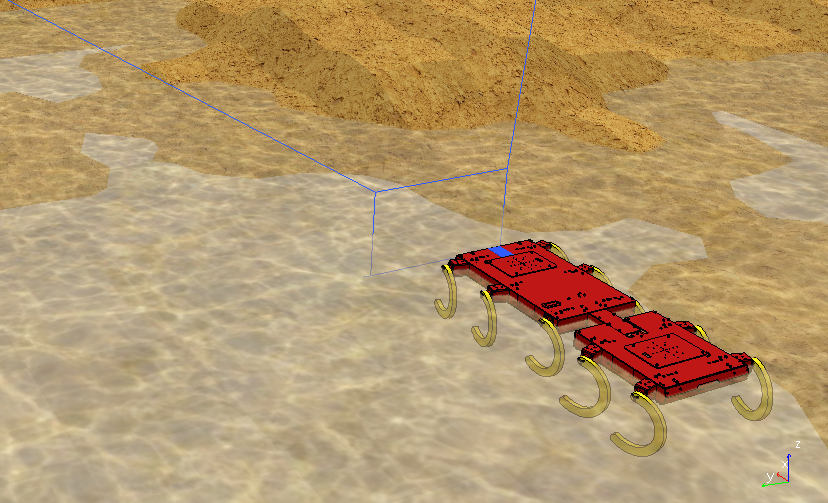
\includegraphics[height=5cm,width=1\textwidth,keepaspectratio]{coppelia_sim.png}
            \caption*{CoppeliaSim simulator, \textbf{4th gen} StriRus}
        \end{subfigure}
        \begin{subfigure}[t]{0.49\textwidth}
            \centering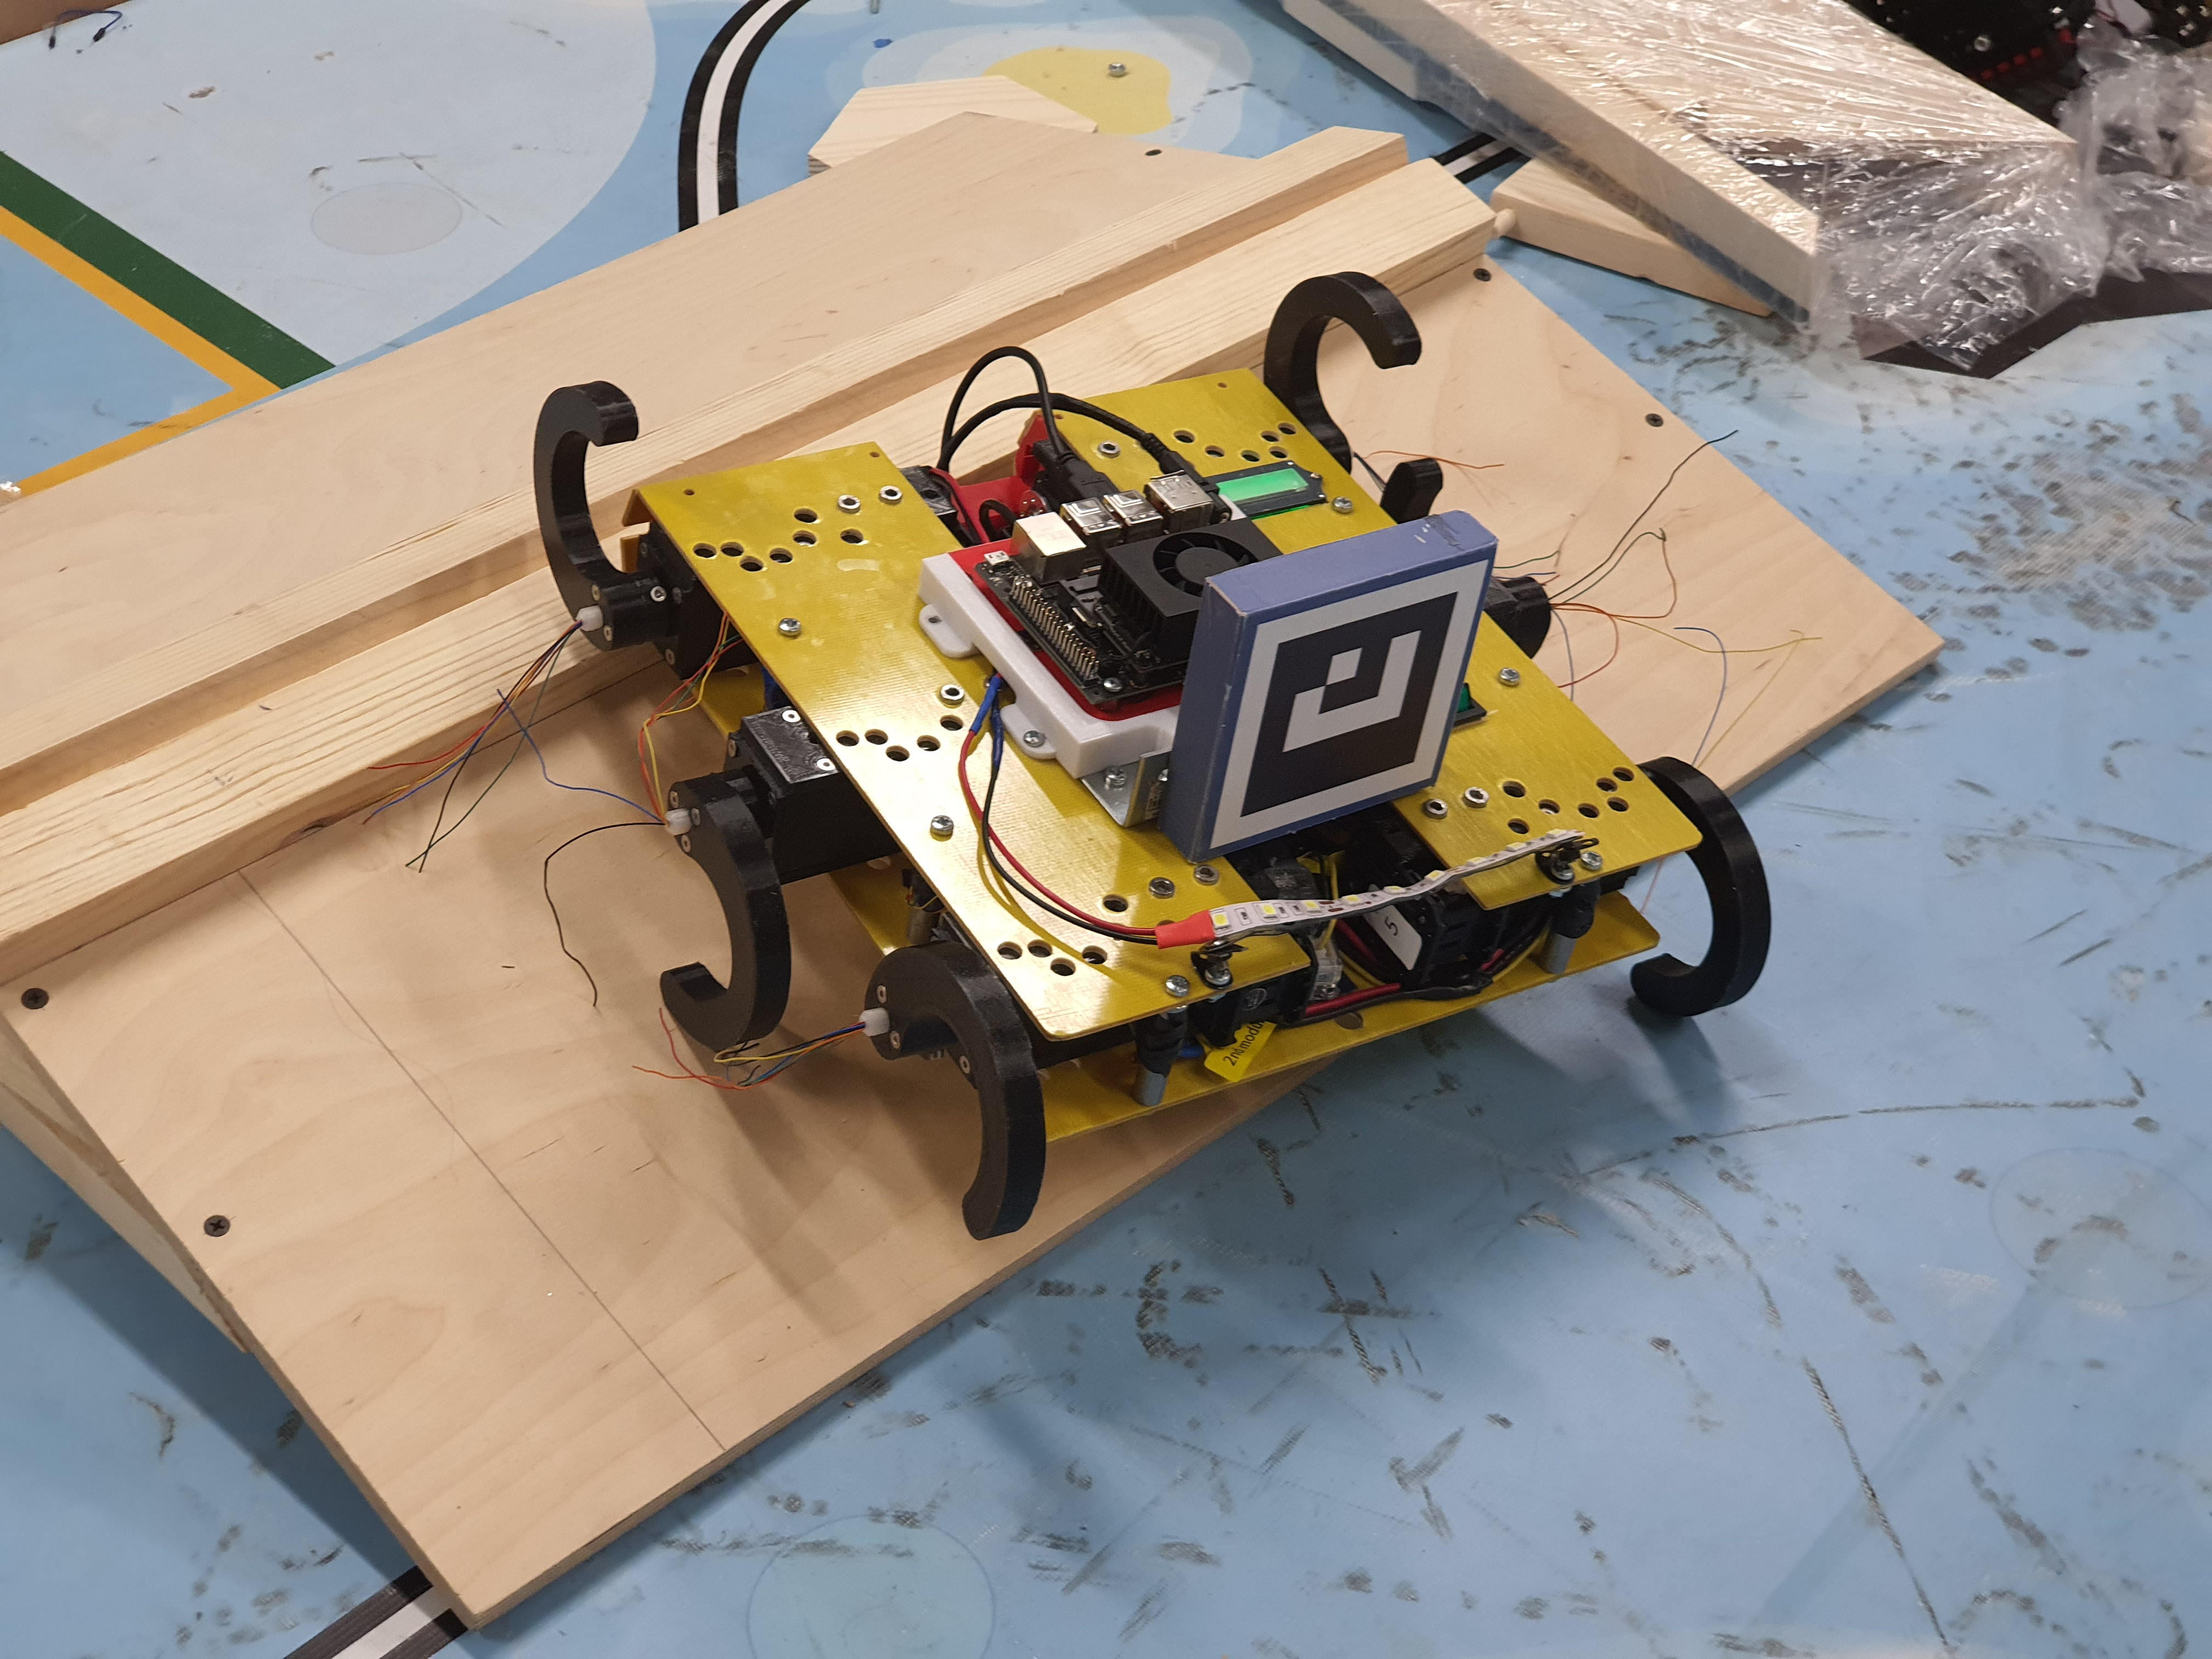
\includegraphics[height=5cm,width=1\textwidth,keepaspectratio]{rl_sim.JPG}
            \caption*{IRL, \textbf{3th+ gen} StriRus}
        \end{subfigure}
    \end{figure}
\end{frame}

\begin{frame}[t]{Map creation based on tactile data}
    \framesubtitle{Assumptions}
    \Large
    Current solution considering such assumptions:
    \begin{itemize}
        \item Our terrain can be represented $z = f(x,y)$. We can use 2D Delaunay triangulation (projected points on a plane)
        \item All simulation data are preprocessed by white noise
    \end{itemize}
\end{frame}

\begin{frame}[t]{Map creation based on tactile data}
    \framesubtitle{Delaunay triangulation}
    \vspace{-0.2cm}
    \begin{figure}[H]
        \centering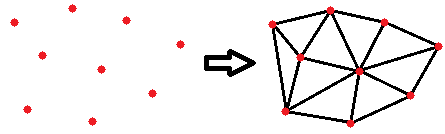
\includegraphics[height=6cm,width=1\textwidth,keepaspectratio]{delone_idea.png}
        \caption*{Common 2D Delaunay triangulation (Convex Hull)}
        \label{fig:delone_idea.png}
    \end{figure}
\end{frame}

\begin{frame}[t]{Map creation based on tactile data}
    \framesubtitle{Result: simulator}
    \vspace{-15pt}
    \begin{figure}[H]
        \begin{subfigure}{0.49\textwidth}
            \centering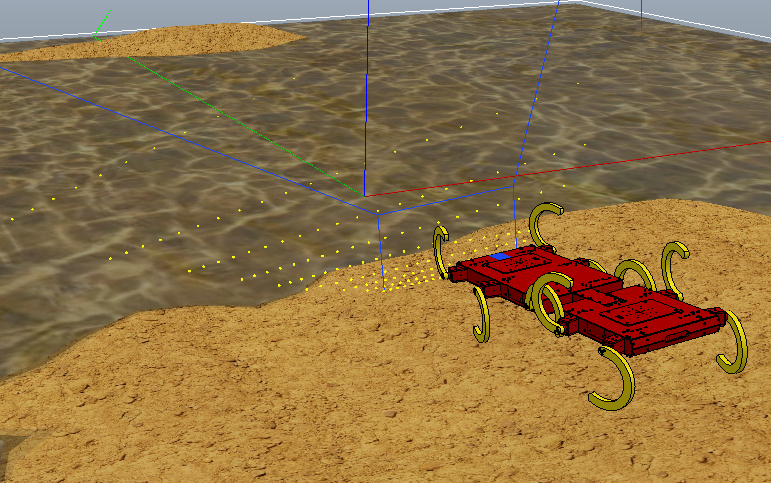
\includegraphics[height=5cm,width=1\textwidth,keepaspectratio]{terrain_w_water1.png}
            \caption*{Start point}
        \end{subfigure}
        \begin{subfigure}{0.49\textwidth}
            \centering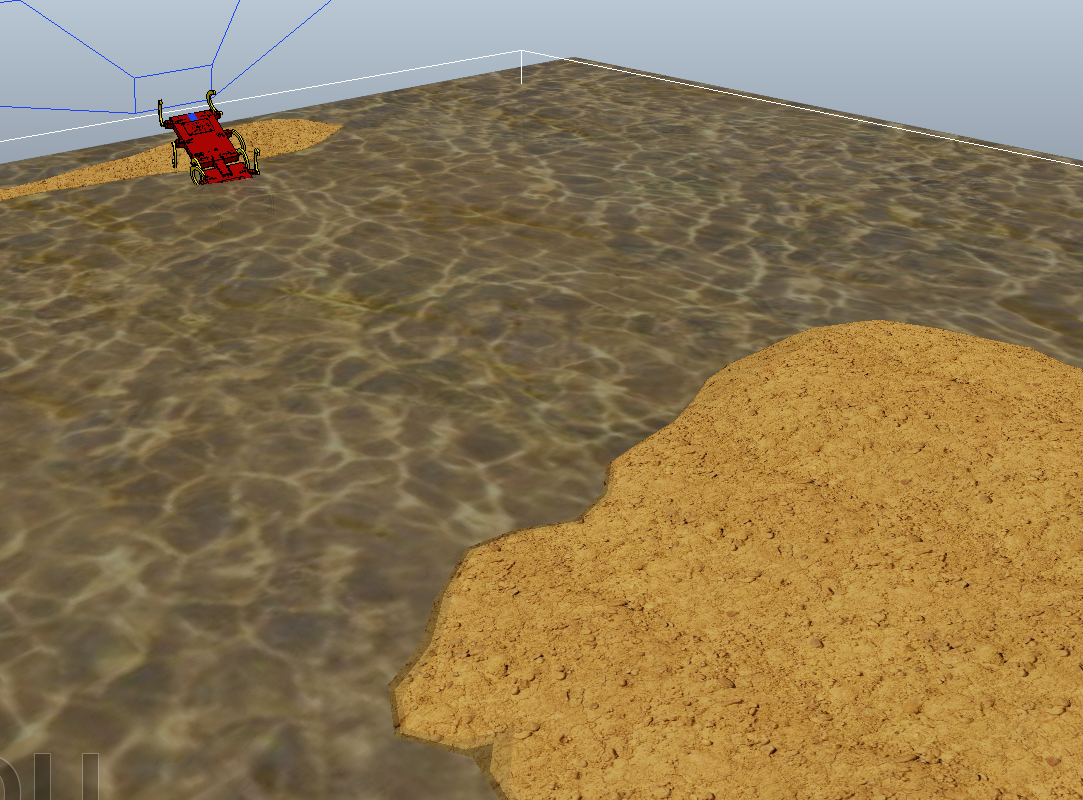
\includegraphics[height=5cm,width=1\textwidth,keepaspectratio]{terrain_w_water_end.png}
            \caption*{End point}
        \end{subfigure}
    \end{figure}
\end{frame}

\begin{frame}[t]{Map creation based on tactile data}
    \framesubtitle{Result: Mesh}
    \vspace{-15pt}
    \begin{figure}[H]
        \begin{subfigure}[t]{0.49\textwidth}
            \centering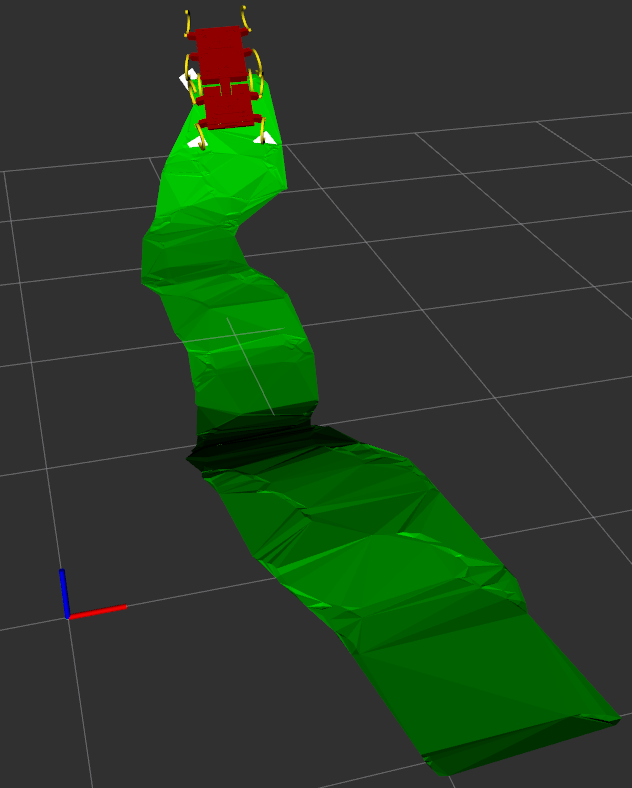
\includegraphics[height=5cm,width=1\textwidth,keepaspectratio]{mesh_rviz.png}
            \caption*{Mesh created using concave hull 2D Delaunay triangulation}
        \end{subfigure}
        \begin{subfigure}[t]{0.49\textwidth}
            \centering\includegraphics[height=5cm,width=1\textwidth,keepaspectratio]{sampled_pcd.png}
            \caption*{Sampled point cloud}
        \end{subfigure}
    \end{figure}
\end{frame}


\begin{frame}[t]{Map creation based on tactile data}
    \framesubtitle{Why do we need a concave hull solution}
    \vspace{-15pt}
    \begin{figure}[H]
        \begin{subfigure}{0.3\textwidth}
            \centering\includegraphics[height=5cm,width=1\textwidth,keepaspectratio]{convex_terr.png}
            \caption*{Case study}
            \label{fig:convex_terr.png}
        \end{subfigure}
        \hfill
        \begin{subfigure}{0.33\textwidth}
            \centering\includegraphics[height=6cm,width=1\textwidth,keepaspectratio]{conv_convex.png}
            \caption*{Convex Hull}
            \label{fig:conv_convex.png}
        \end{subfigure}
        \hfill
        \begin{subfigure}{0.33\textwidth}
            \centering\includegraphics[height=6cm,width=1\textwidth,keepaspectratio]{conv_concave.png}
            \caption*{Concave Hull}
            \label{fig:conv_concave.png}
        \end{subfigure}

    \end{figure}
\end{frame}

\begin{frame}[t]{Map creation based on tactile data}
    \framesubtitle{Metric: point cloud comparison with ground truth}
    \vspace{-15pt}
    \begin{figure}[H]
        \begin{subfigure}[t]{0.49\textwidth}
            \centering\includegraphics[height=5cm,width=1\textwidth,keepaspectratio]{cropped_pcd.png}
            \caption*{Overlaid point clouds}
        \end{subfigure}
        \begin{subfigure}[t]{0.49\textwidth}
            \centering\includegraphics[height=5cm,width=1\textwidth,keepaspectratio]{pcd_hist.png}
            \caption*{Error histogram (distance from a point to closest ground truth point)}
        \end{subfigure}
    \end{figure}
    % \alert{\Large RMSE 0.053074, std 0.025}
\end{frame}

\begin{frame}[t]{Map creation based on tactile data}
    \framesubtitle{Metric: mesh comparison with ground truth}
    \vspace{-15pt}
    \begin{figure}[H]
        \begin{subfigure}[t]{0.49\textwidth}
            \centering\includegraphics[height=5cm,width=1\textwidth,keepaspectratio]{mesh_comp.png}
            \caption*{Overlaid meshes}
        \end{subfigure}
        \begin{subfigure}[t]{0.49\textwidth}
            \centering\includegraphics[height=5cm,width=1\textwidth,keepaspectratio]{mesh_hist.png}
            \caption*{Error histogram (distance from a point to closest ground truth point)}
        \end{subfigure}
    \end{figure}
    % \alert{\Large RMSE 0.00167067, std 0.0005}
\end{frame}

\begin{frame}[t]{Map creation based on tactile data}
    \framesubtitle{Result: real world experiment, video}
    \vspace{-0.5cm}
    \begin{figure}[H]
        \begin{subfigure}[t]{0.49\textwidth}
            \href{run:./videos/big_angle2.mp4}{
                \centering\includegraphics[height=6cm,width=1\textwidth,keepaspectratio]{real_robot_mesh_video_preview.png}}
            \caption*{Robot is passing the obstacle}
        \end{subfigure}
        \begin{subfigure}[t]{0.49\textwidth}
            \centering\includegraphics[height=6cm,width=1\textwidth,keepaspectratio]{real_mesh.jpg}
            \caption*{Mesh, obtained from legs}
        \end{subfigure}
    \end{figure}
\end{frame}

\begin{frame}[t]{Map creation based on tactile data}
    \framesubtitle{Summary}
    \Large
    \begin{itemize}
        \item Map can be built using concave hull 2D Delaunay triangulation.

              A Sparse point cloud obtained from force sensors, installed on legs.
        \item \textit{Simulator}: \begin{itemize}
                  \item Avg. Point cloud comparison RMSE is about 5 cm.
                  \item Avg. Mesh comparison RMSE is about 1 cm.
              \end{itemize}
        \item \textit{Real world experiment}: \begin{itemize}
                  \item Avg. Point cloud comparison RMSE is about 8 cm.
                        %     \item Avg. Mesh comparison RMSE is about 1 cm.
              \end{itemize}
    \end{itemize}
\end{frame}

\begin{frame}[t]{Summary}
    \framesubtitle{}
    \Large
    \begin{itemize}
        \item Robot was created
        \item Force transducer based on Velostat was created and was investigated
        \item Robot can distinct rubber and rock terrains
        \item Robot can build a map using tactile sensors
    \end{itemize}
\end{frame}

% \fbckg{fibeamer/figs/last_page.png}
% \frame[plain]{}
% \fbckg{fibeamer/figs/common.png}

\end{document}